\chapter{Geometry in Vector Spaces}
Vector spaces give a rich environment to explore the relationships between 
objects and gives natural abstractions to other types of {\it vectors} (e.g. functions,
matrices, polynimials, etc).  Most of the study of vector spaces involves abstraction
and making precise ideas that spanned many decades, or centuries, in many different fields
of science and mathematics.  In this sense, the study of vector spaces leans heavily on
past mathematical results and seeks to give them order and structure.  You
have seen that the study of vector spaces really acts as a unifying language to talk about
a wide variety of mathematical objects.

In this chapter we layer the language of abstract vector spaces and the language of
geometry.  In particular, we will build and abstract the familiar ideas of angle,
othogonality, lengths of vectors, and distance in general vector spaces.  We will make
precise the ideas of the {\it size of a function} or the {\it distance between two
matrices} or {\it polynomials}.  These notions are likely second nature in our familiar
vector spaces 
$\mathbb{R}^2$ and $\mathbb{R}^3$, but what about in spaces of matrices? spaces of
functions? spaces of polynomials?  The notions of angle and  distance can be abstracted in
a natural and beautiful way so that our intuitive ideas still hold, but we also get
something mathematically meaningful in the more abstract spaces.  We'll start with an idea
that is probably familiar to you: the dot product\footnote{If you haven't had
multivariable calculus or calculus-based physics then maybe the idea of a dot product will
be new to you.  Don't worry.  We'll introduce everything from scratch here.}.  From the
dot product we will build a similar idea is more general vector spaces so that the ideas
of angle and perpendicularity come along for the ride.  Here we go!

\section{The Geometry of Euclidean Space}
At this point we have talked almost exclusively about linear combinations and the spaces
associated with them.  We have not, however, discussed the geometry of vector spaces.  So
far we haven't generalized the notions of angle and length of vectors to our large view of
vector spaces.  You may recall things like projections, angles, norms (lengths) from
$\mathbb{R}^2$ or $\mathbb{R}^3$ as discussed in physics or in multivariable calculus but
you need to keep in mind that this is only a limited view of the world of vector spaces.
Let's jump right in by filling in some definitions and theorems that you likely already
know

\subsection{The Dot Product}
The following are two different familiar definitions of the dot product.  The first gives
a purely algebraic formula for the dot product and the second gives a more geometric
definition.  They are indeed equivalent definitions.
\begin{definition}[Algebraic Dot Product in $\mathbb{R}^n$]
    Let $\bu, \bv \in \mathbb{R}^n$.  The {\bf dot product} of $\bu$ and $\bv$ is defined
    algebraically as
    \[ \bu \cdot \bv = u_1 v_1 + u_2 v_2 + \cdots + u_n v_n = \sum_{j=1}^n u_j v_j. \]
    Notice that this definition doesn't explicitly mention the angle between the vectors.
\end{definition}
% \solution{
%     $\bu \cdot \bv = \sum_{j=1}^n u_j v_j$
% }

\begin{definition}[Geometric Dot Product in $\mathbb{R}^n$]
    If $\bu,\bv\in\mathbb{R}^n$ then the relationship between the dot product of the
    vectors and the angle between the vectors is
    \[ \bu \cdot \bv = \|\bu\| \|\bv\| \cos \theta. \]
    Notice that if you want the angle between two vectors then 
    \[ \theta = \cos^{-1} \left( \frac{\bu \cdot \bv}{\| \bu \| \|\bv\|} \right). \]
\end{definition}
One should note that the angle formula only holds if both $\|\bu\|\ne0$ and $\|\bv\|\ne0$.

Now we build the mathematical notation for orthogonality and length of vectors in
$\mathbb{R}^n$.  Both of these geometric concepts are build upon the dot product.
\begin{definition}[Orthogonal Vectors]
    Two vectors are said to be orthogonal (perpendicular) if their dot product is zero.
\end{definition}
\begin{problem}
    Use the geometric definition of the dot product to prove that statements 
    \begin{itemize}
        \item ``the dot product of two vectors is zero'', and 
        \item ``the vectors are perpendicular'' 
    \end{itemize}
    are indeed the same based on your familiar understanding of what ``perpendicular''
    means.
\end{problem}
% \begin{thm}[Orthogonal Vectors in $\mathbb{R}^n$]
%     If $\bu,\bv\in\mathbb{R}^n$ then $\bu$ is orthogonal (perpendicular) to $\bv$ if and
%     only if \underline{\hspace{1in}}.
% \end{thm}
% \solution{
% $\bu \cdot \bv = 0$
% }
% \begin{proof}
%     (prove this theorem)
% \end{proof}
\solution{
$\bu \cdot \bv = \|\bv \| \|\bu\| \cos \theta$ and if $\theta = \pi/2$ we know that
$\cos \theta = 0$.  Hence $\bu \cdot \bv = 0$.
}

\begin{definition}[Length of Vectors in $\mathbb{R}^n$]
    Let $\bu \in \mathbb{R}^n$.  The {\bf length (norm)} of $\bu$ is
    \[ \| \bu \| = \sqrt{\bu \cdot \bu} = \underline{\hspace{2in}} \]
    (fill in the blank using the algebraic definition of the dot product)
\end{definition}
\solution{
    $\|\bu\| = \sum_{j=1}^n u_j^2$
}

\begin{problem}
    If $\bu,\bv \in \mathbb{R}^2$ then what familiar theorem do you see in the definition
    of the length of a vector?  Another way to put this is: the definition of the length
    of a vector in $\mathbb{R}^n$ is a generalization of what familiar theorem?
\end{problem}
\solution{
    This is just Pythagorean Theorem.
}

\begin{definition}[Distance Between Vectors in $\mathbb{R}^n$]
    Let $\bu,\bv\in\mathbb{R}^n$.  The {\bf distance between} $\bu$ and $\bv$ is
    \[ \text{dist}(\bu,\bv) = \| \bu - \bv\| = \underline{\hspace{1in}} \]
    (fill in the blank)
\end{definition}
\solution{
    $\text{dist}(\bu,\bv) = \|\bu-\bv\|$
}

\begin{definition}[Unit Vectors in $\mathbb{R}^n$]
    Let $\bv \in \mathbb{R}^n$.  We say that $\bv$ is a unit vector if $\|\bv\| = 1$.  If
    you have a vector $\bv$ that is not a unit vector (has length other than 1) then you
    can scale it to become a unit vector by dividing by its length
    \[ (\text{unit vector in the direction of $\bv$}) = \bu = \frac{\bv}{\|\bv\|}. \]
\end{definition}

OK.  Most of the geometric players are on the table: angle, distance, length, and
perpendicularity.  Here we give a straight forward example showing how to use these ideas
in $\mathbb{R}^3$.


\begin{problem}
    Let $\bu$ and $\bv$ be defined as.  Find $\bu \cdot \bv$, $\|\bu\|$, $\|\bv\|$, and
    the angle between them.
    \[ \bu = \left( \begin{array}{c} 0 \\ 1 \\ -1 \end{array} \right) \]
    \[ \bv = \left( \begin{array}{c} 4 \\ 2 \\ -3 \end{array} \right) \]
% 
% \begin{enumerate}
%     \item[(a)] 
% $\left( \begin{array}{c} 0 \\ 2 \\ 3 \end{array} \right)$
% \item[(b)] 5
% \item[(c)] 0
% \item[(d)] The dot product cannot be computed for these vectors.
% \end{enumerate}
\end{problem}
% \begin{problem}
%     \begin{itemize}
%             \input{ClickerQuestions/LA.00.22.010}
%     \end{itemize}
% \end{problem}
\solution{
The dot product is $(0)(4) + (1)(2) + (-1)(-3) = 2+3 = 5$
}
\begin{example}
    Let $\bu, \bv \in \mathbb{R}^3$ be defined as
    \[ \bu = \begin{pmatrix} 2 \\ -1 \\ 4 \end{pmatrix} \quad \text{and} \quad \bv =
    \begin{pmatrix} 0 \\ 9 \\ -3 \end{pmatrix} \]
    What are $\bu \cdot \bv$, $\|\bu\|$, $\|\bv\|$, and $\text{dist}(\bu,\bv)$?  Are the
    two vectors orthogonal?   What is the angle between them? \\ {\bf
    Solution:} 
    \begin{flalign*}
        \bu \cdot \bv &= (2)(0) + (-1)(9) + (4)(-3) = -9 - 12 = -21 \\
        \|\bu\| &= \sqrt{2^2 + (-1)^1 + 4^2} = \sqrt{4 + 1 + 16} = \sqrt{21} \\
        \|\bv\| &= \sqrt{0^2 + 9^2 + (-3)^2} = \sqrt{81 + 9} = \sqrt{90} \\
        \text{dist}(\bu,\bv) &= \| \bu - \bv\| = \| \begin{pmatrix} 2 \\ -10 \\ 7
        \end{pmatrix} \| = \sqrt{4+100+49} = \sqrt{153}.
    \end{flalign*}
    The vectors are not orthogonal since $\bu \cdot \bv \ne 0$.  The angle between the
    vectors is 
    \[ \theta = \cos^{-1} \left( \frac{\bu \cdot \bv}{\|\bu\| \|\bv\|} \right) =
    \cos^{-1}\left( \frac{-21}{\sqrt{21}\sqrt{90}} \right) \]
\end{example}


\subsection{Projections}
Finally we are going to discuss projections.  When dealing with projections you should be
thinking about how shadows are cast between vectors.  To solidify this notion (even though
you likely already know it) let's look at some projections in $\mathbb{R}^2$ before we
ramp up the dimension.  Take a look at Figure \ref{fig:proj_R2}.  We would like to project
vector $\bu$ onto vector $\bv$ and by that we mean that we would like to draw a vector
(depicted by the dashed vector $\bw$ in the figure) that is perpendicular to $\bv$ and meets the
head of $\bu$. This projection creates the vector $\hat{\bv}$ so that $\hat{\bv}$ points
in exactly the same direction as $\bv$ but $\hat{\bv} \perp \bw$. Since $\bv$ and
$\hat{\bv}$ point in the same direction we know that $\hat{\bv} = c\bv$ for some scalar
$c$.  Furthermore, we know that $\bw + \hat{\bv} = \bu$ so $\bw = \bu - \hat{\bv}$. Therefore,
\begin{flalign*}
    &0 = \hat{\bv} \cdot \bw = c\bv \cdot \left( \bu - c\bv \right) \\
    &\implies c\bv \cdot \bu - c^2 \bv \cdot \bv = 0 \\
    &\implies \bu \cdot \bv = c \bv \cdot \bv \\
    &\implies c = \frac{\bu \cdot \bv}{\bv \cdot \bv}
\end{flalign*}
\begin{figure}[ht!]
    \begin{center}
        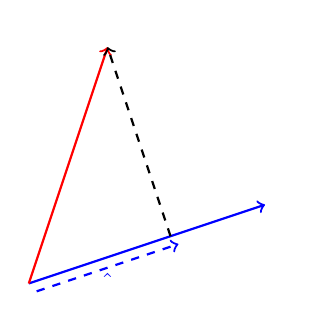
\begin{tikzpicture}
            \draw[->,thick, blue] (0,0) -- (3,1) node[anchor=west]{$\bv$};
            \draw[->,thick, red] (0,0) -- (1,3) node[anchor=south]{$\bu$};
            \draw[->,thick, dashed, black] (1.8,0.6) -- (1,3);
            \draw[black] (1.4,2) node[anchor=west]{$\bw$};
            \draw[->,thick, dashed, blue] (0.1,-0.1) -- (1.9,0.5);
            \draw[blue] (1,0.25) node[anchor=north]{$\hat{\bv}$};
        \end{tikzpicture}
    \end{center}
    \caption{Depiction of vector projection in $\mathbb{R}^2$.}
    \label{fig:proj_R2}
\end{figure}

All of the prior discuss proves the following theorem but notice that we never made any
mention explicitly about the vectors living in $\mathbb{R}^2$.  In fact, the proof that we
gave works generally in $\mathbb{R}^n$.
\begin{thm}[Orthogonal Projection]
    Let $\bu, \bv \in \mathbb{R}^n$.  If we are to project $\bu$ onto $\bv$ as in Figure
    \ref{fig:proj_R2} we get
    \begin{flalign*}
        \text{proj}_{\bv}(\bu) &= \hat{\bv} = \left( \frac{\bv \cdot \bu}{\bv \cdot \bv}
        \right) \bv =
        \text{projection of $\bu$ onto $\bv$} \\
        \bw &= \bu - \hat{\bv} = \bu - \left( \frac{\bv \cdot \bu}{\bv \cdot \bv} \right)
        \bv
        = \text{projection error}
    \end{flalign*}
    The vector $\bw$ is often called the {\it error} in the projection.
\end{thm}



\begin{problem}
    If $\bb = \left( \begin{array}{c} 3 \\ -1  \end{array} \right)$ and $y = \left(
    \begin{array}{c} 2 \\ 1  \end{array} \right),$ then what is the orthogonal projection of $\bb$
    onto $\by$?  Find your solution analytically and draw of graph depicting your answer.
% 
% \begin{enumerate}
%     \item[(a)] $\left( \begin{array}{c} 2 \\ 1  \end{array} \right)$
%     \item[(b)] $\left( \begin{array}{c} 3/2 \\ -1/2 \end{array} \right)$
%     \item[(c)] $\left( \begin{array}{c} 10 \\ 5  \end{array} \right)$
%     \item[(d)] $\left( \begin{array}{c} 1/10 \\ 3/10  \end{array} \right)$
% \end{enumerate}
% 
\end{problem}
% \begin{problem}
%     \begin{itemize}
%             \input{ClickerQuestions/LA.00.24.010}
%     \end{itemize}
% \end{problem}
\solution{
    $\text{proj}_y b = \left( \frac{b \cdot y}{y \dot y} \right) y = \left(
    \frac{5}{5}
    \right) \begin{pmatrix} 2 \\ 1 \end{pmatrix} = \begin{pmatrix}2\\1\end{pmatrix}$
}

We know what a basis is and what know what orthogonal vectors are.  If you think carefully
about it, all of your mathematical life you have been dealing with coordinate systems that have
orthogonal bases.  Every time you graph in $\mathbb{R}^2$ or $\mathbb{R}^3$ you've used
the idea of othogonality without thinking much about it.  Let's see why this is so
incredibly useful.

\begin{problem}
    If $\mathcal{B} = \{\bv_1, \bv_2, \ldots, \bv_n\}$ is an orthogonal basis for a vector
    space $\mathcal{V}$ then how do you write $\bx$ as a linear combination of the basis vectors?\\
    (Why is it advantageous to have an orthogonal basis?) 
    Hint: Since $\bx = c_1 \bv_1 + c_2 \bv_2 + \cdots + c_n \bv_n$ how can you use
    orthogonality to solve for $c_j$?
\end{problem}
\solution{
    $c_j = \frac{\bx \cdot \bv_j}{\bv_j \cdot \bv_j}$
}

\begin{problem}
    Implement your idea on the subspace spanned by the basis
    \[ \mathcal{B} = \left\{ \begin{pmatrix} 1\\4\\-3 \end{pmatrix}\, , \, \begin{pmatrix}
            3 \\ 0 \\ 1 \end{pmatrix} \right\} \]
    where $\bx$ is in the subspace of $\mathbb{R}^3$ spanned by $\mathcal{B}$.
    Specifically, let $\bx$ be defined as
    \[ \bx = \begin{pmatrix} 2 \\ -4\\ 1 \end{pmatrix} \]
\end{problem}
\solution{
    Since $\bx = c_1 \begin{pmatrix} 1 \\ 4 \\ -3 \end{pmatrix} + c_2 \begin{pmatrix} 3 \\ 0 \\
        1 \end{pmatrix}$ so 
    \[ c_1 = \frac{\bx \cdot \bv_1}{\bv_1 \cdot \bv_1} = \frac{-17}{26} \]
    \[ c_2 = \frac{\bx \cdot \bv_2}{\bv_2 \cdot \bv_2} = \frac{7}{10} \]
}

Now summarize the process that you built in the previous problem into the following
theorem.
\begin{thm}[Building Vectors from an Orthogonal Basis]\label{thm:orthogonal_basis}
    If $\mathcal{B} = \{\bv_1, \bv_2, \ldots, \bv_n\}$ is an orthogonal basis for a vector
    space $\mathcal{V}$ then for any vector $\bx \in \mathcal{V}$ we can write
    \[ \bx = C_1 \bv_1 + C_2 \bv_2 + \cdots + C_n \bv_n \]
    where
    \[ C_k = \underline{\hspace{1in}}. \]
%     \[ \bx = \underline{\hspace{0.25in}} \bv_1 + \underline{\hspace{0.25in}} \bv_2 +
%     \underline{\hspace{0.25in}} \bv_3 + \cdots + \underline{\hspace{0.25in}} \bv_n \]
%     (Fill in the blanks)
\end{thm}
\begin{proof}
    (prove this theorem by leveraging the fact that we have an orthogonal basis)
\end{proof}
\solution{
    $c_j = \frac{\bx \cdot \bv_j}{\bv_j \cdot \bv_j}$
}


\begin{thm}
    If the nonzero vectors $\bu_1, \bu_2, \bu_3, \dots, \bu_k$ are mutually orthogonal
    then they are linearly independent.
\end{thm}
\begin{proof}
    (prove this theorem)
\end{proof}
\solution{
    Consider $\bo = \sum_{j=1}^n c_j \bu_j$.  From the previous theorem we know that $c_j
    = (\bo \cdot \bu_j) / (\bu_j \cdot \bu_j) = 0$.  Therefore the only solution is the
    trivial solution and the vectors must be linearly independent.
}


\begin{problem}
    Determine if the following set of vectors is linearly independent.  Do this two
    different ways.
    \[ \left\{ \begin{pmatrix} 3 \\ 1 \\ 1 \end{pmatrix} \, , \, \begin{pmatrix} -1 \\ 2
            \\ 1
    \end{pmatrix} \, , \, \begin{pmatrix} -1 \\ -4 \\ 7 \end{pmatrix} \right\} \]
\end{problem}
\solution{
They are mutually orthogonal so they are linearly independent.
}







\begin{problem}
    If we have two linearly independent vectors that are NOT orthogonal, how do
    we find a set of two orthogonal vectors that span the same space?

    For example, can we find two orthogonal vectors that span the same space as
    \[ \begin{pmatrix} 2 \\ 0 \end{pmatrix} \quad \text{and} \quad \begin{pmatrix} 1
        \\ 1 \end{pmatrix} \]
\end{problem}

\subsection{The Gram-Schmidt Process: Making Orthogonal Sets}
The previous theorems and problems give us good reason to think that having an orthogonal
(or orthonormal) basis for a vector space is advantageous both computationally and
geometrically.  In fact, we have been used to an orthonormal basis all of our matheamtical
lives since that is what the regular Cartesian coordinate system is built from.  The
question now is this: \\
Given a basis $\mathcal{B}$ for a vector space $\mathcal{V}$ how can we transform that
basis into a different basis for the same space but also gain orthogonality?
We will build your intuition to the process via a scaffolded problem.  

\begin{problem}
    Build a basis for $\mathbb{R}^2$ so that it contains two orthogonal unit vectors with
    one of the vectors parallel to $\bv_1 = \begin{pmatrix} 1\\1\end{pmatrix}$.
\end{problem}

\begin{problem}
    Consider the vector space $\mathbb{R}^3$ with the basis $\mathcal{B} = \{\bv_1, \bv_2,
    \bv_3\}$ given by
    \[ \bv_1 = \begin{pmatrix} 1\\1\\1\end{pmatrix}, \quad \bv_2 = \begin{pmatrix} 0
            \\1\\1\end{pmatrix},\quad \bv_3 = \begin{pmatrix} 0\\0\\1\end{pmatrix} \]
                We are going to build a basis $\mathcal{U} = \{\bu_1, \bu_2, \bu_3\}$ such that $\text{span}(\mathcal{U}) =
    \mathbb{R}^3$ but the vectors are also mutually orthogonal and all have unit length.
    (One should note here that the normalization step is optional but since unit vectors
    are so nice to work with we are leaving it here.)
    \begin{enumerate}
        \item[(a)] Define $\bu_1$ as a unit vector that points in the same direction as
            $\bv_1$.
            \[ \bu_1 = \frac{1}{\|\bv_1\|} \bv_1 =  \begin{pmatrix} \underline{\hspace{0.25in}} \\
                    \underline{\hspace{0.25in}} \\ \underline{\hspace{0.25in}} \end{pmatrix}
                    \]
\solution{
    $\bu_1 = \frac{1}{\sqrt{3}} \begin{pmatrix} 1\\1\\1\end{pmatrix} = \begin{pmatrix}
        1/\sqrt{3} \\ 1/\sqrt{3} \\ 1/\sqrt{3} \end{pmatrix}$
}
        \item[(b)] Now we project $\bv_2$ onto $\bu_1$ and find the error in the
            projection.  This would be the vector $\bw$ in Figure \ref{fig:proj_R2}.  Once
            we have the error we should normalize it to get $\bu_2$.
            \[ \bw_2 = \bv_2 - \text{proj}_{\bu}(\bv_2) = \bv_2 - \left( \bv_2 \cdot \bu_1
                \right) \bu_1 \quad \text{and therefore} \quad \bu_2 =
                \frac{1}{\|\bw_2\|}\bw_2. \]
            Draw a picture of what we just did.
            \[ \bu_2 = \frac{1}{\|\bv_1\|} \bv_1 =  \begin{pmatrix}
                    \underline{\hspace{0.25in}} \\ \underline{\hspace{0.25in}} \\
                    \underline{\hspace{0.25in}} \end{pmatrix} \]
\solution{
    $\bw_2 = \begin{pmatrix} 0\\1\\1\end{pmatrix} - \left( \frac{2}{\sqrt{3}}
        \right)\begin{pmatrix} 1/\sqrt{3} \\ 1/\sqrt{3} \\ 1/\sqrt{3} \end{pmatrix} =
            \begin{pmatrix}0\\1\\1\end{pmatrix} - \begin{pmatrix} 2/3 \\ 2/3 \\ 2/3
            \end{pmatrix} = \begin{pmatrix} -2/3 \\ 1/3 \\ 1/3 \end{pmatrix}$.  Therefore
                $\bu_2 = \frac{1}{\|\bw_2\|}\bw_2 $ so
                \[ \bu_2 = \frac{\sqrt{3}}{\sqrt{2}} \begin{pmatrix} -2/3 \\ 1/3 \\
                        1/3\end{pmatrix} = \frac{1}{\sqrt{6}} \begin{pmatrix}
                            -2\\1\\1\end{pmatrix} = \begin{pmatrix} -2/\sqrt{6} \\
                                1/\sqrt{6} \\ 1/\sqrt{6} \end{pmatrix} \]
}
        \item[(c)] For $\bu_3$ we project $\bv_3$ onto both $\bu_1$ and $\bu_2$ and then
            normalize.
            \[ \bw_3 = \bv_3 - \left( \bv_3 \cdot \bu_1 \right)\bu_1 - \left( \bv_3 \cdot
                \bu_2
                \right) \bu_2 \quad \text{and therefore} \quad \bu_3 =
                \frac{1}{\|\bw_3\|}\bw_3 \]
            \[ \bu_3 = \frac{1}{\|\bv_1\|} \bv_1 =  \begin{pmatrix}
                    \underline{\hspace{0.25in}} \\ \underline{\hspace{0.25in}} \\
                    \underline{\hspace{0.25in}} \end{pmatrix} \]
\solution{
    \[ \bw_3 = \bv_3 - \left( \frac{1}{\sqrt{3}} \right)\begin{pmatrix} 1/\sqrt{3} \\
            1/\sqrt{3} \\ 1/\sqrt{3} \end{pmatrix} - \left( \frac{1}{\sqrt{6}} \right)
            \begin{pmatrix} -2/\sqrt{6} \\ 1/\sqrt{6} \\ 1/\sqrt{6} \end{pmatrix} =
                \begin{pmatrix}0\\0\\1\end{pmatrix} - \begin{pmatrix}1/3 \\ 1/3 \\ 1/3
                \end{pmatrix} - \begin{pmatrix} -2/6 \\ 1/6 \\ 1/6 \end{pmatrix} =
                    \begin{pmatrix} 0 \\ -1/2 \\ 1/2 \end{pmatrix} =
                        \frac{1}{2} \begin{pmatrix}0\\-1\\1\end{pmatrix} \]
    Therefore, we can build $\bu_3$ by normalizing
    \[ \bu_3 = \frac{\sqrt{2}}{2} \begin{pmatrix} 0\\-1\\1 \end{pmatrix}  =
            \frac{1}{\sqrt{2}} \begin{pmatrix} 0\\-1\\1\end{pmatrix} = \begin{pmatrix}
                0\\-1/\sqrt{2} \\ 1/\sqrt{2} \end{pmatrix}\]
}
        \item[(d)] Verify that indeed $\mathcal{U} = \{\bu_1, \bu_2, \bu_3\}$ is an
            orthonormal basis for $\mathbb{R}^3$.
\solution{
The orthonormal basis is:
\[ \mathcal{U} = \left\{ \begin{pmatrix} 1/\sqrt{3} \\ 1/\sqrt{3} \\ 1/\sqrt{3}
    \end{pmatrix} \, , \, \begin{pmatrix} -2/\sqrt{6} \\ 1/\sqrt{6} \\ 1/\sqrt{6}
    \end{pmatrix} \, , \, \begin{pmatrix} 0 \\ -1/\sqrt{2} \\ 1/\sqrt{2} \end{pmatrix}
    \right\} \]
    and we leave it to the reader to verify that indeed the vectors are mutually
    orthogonal.
}
    \end{enumerate}
\end{problem}


\begin{problem}
    Use the Gram-Schmidt process outlined in the previous problem to produce an orthogonal
    basis $\mathcal{U}$ for the subspace spanned by
    \[ \begin{pmatrix} 3\\0\\-1\end{pmatrix} \quad \text{and} \quad \begin{pmatrix}
            8\\5\\-6\end{pmatrix}. \]
\end{problem}

\begin{problem}
    Let's build an orthogonal basis $\mathcal{U}$ for $\mathbb{R}^3$.  To get started let
    $\bu_1 = \begin{pmatrix} 1\\0\\1\end{pmatrix}$.  (notice that we are not
        normalizing this time)
        \begin{enumerate}
            \item[(a)] Create a vector $\bu_2$ in $\mathbb{R}^3$ so that $\bu_1 \perp
                \bu_2$.
\solution{
A simple choice is $\bu_2 = (0,1,0)^T$.
}
            \item[(b)] Pick a vector $\bv_3 \in \mathbb{R}^3$ such that $\bv_3$ is
                linearly independent of $\bu_1$ and $\bu_2$.  Then use one step of the
                Gram-Schmidt process to create $\bu_3$ out of $\bv_3$.
\solution{One choice is $\bv_3 = (2,0,1)^T$.  Therefore
    \[ \bu_3 = \bv_3 - \left( \frac{\bv_3 \cdot \bu_1}{\|\bu_1\|^2} \right)\bu_1 - \left(
        \frac{\bv_3 \cdot \bu_2}{\|\bu_2\|^2}\right) \bu_2 = \begin{pmatrix}
            2\\0\\1\end{pmatrix} - \frac{3}{2}\begin{pmatrix} 1\\0\\1\end{pmatrix} - 0
                \begin{pmatrix} 0\\1\\0\end{pmatrix} = \begin{pmatrix} 1/2 \\ 0 \\
                    -1/2\end{pmatrix} \]
}
            \item[(c)] Verify that the vectors in your proposed basis are indeed mutually
                orthogonal.  If so we can use one of the previous theorems (which one) to
                say that the vectors are linearly independent and must therefore span
                $\mathbb{R}^3$.
\solution{It is trivial to verify that the three vectors are indeed mutually orthogonal.
}
        \end{enumerate}
\end{problem}


\newpage\section{Inner Product Spaces}
Now time for some more abstraction!  In this section we take the notions of geometry and
abstract them to generalized vector spaces.  You may have noticed that the dot product is
the basic computation necessary to understand angle in $\mathbb{R}^n$ so we first have to
provide a generalized version of the dot product.

\begin{definition}[The Inner Product]\label{def:inner_product}
    An {\bf inner product} is the abstraction of a dot product to a general vector space.
    If $\bu$, $\bv$, and $\bw$ are vectors in a vector space $\mathcal{V}$ and $c$ is some real
    number then
        \begin{enumerate}
            \item $\left< \bu,\bv\right> = \left<\bv,\bu\right>$
            \item $\left< \bu,\bv + \bw\right> = \left< \bu,\bv\right> + \left<
                \bu,\bw\right>$
            \item $\left< c\bu,\bv\right> = c \left< \bu,\bv\right>$
            \item $\left< \bu,\bu\right> \ge 0$ and $\left<\bu,\bu\right>=0$ if and only if
                $\bu=\bo$
        \end{enumerate}
\end{definition}

\begin{problem}
    Verify that the dot product is indeed an inner product on the vector space
    $\mathbb{R}^n$. 
\end{problem}
\solution{
    \begin{enumerate}
        \item The dot product is definitely symmetric: $\bu \cdot \bv = \bv \cdot \bu$.
            Proof:
            \[ \bu \cdot \bv = \sum_{j=1}^n u_j v_j = \sum_{j=1}^n v_j u_j = \bv \cdot \bu
            \]
    \item $\bu \cdot (\bv + \bw) = (\bu \cdot \bv) + (\bu + \bw)$ since
        \[ \bu \cdot (\bv + \bw) = \sum_{j=1}^n u_j(v_j+w_j) = \sum_{j=1}^n u_j v_j + u_j
            w_j = \sum_{j=1}^n u_j v_j + \sum_{j=1}^n u_j w_j = \bu \cdot \bv + \bu \cdot
        \bw \]
    \item $(c\bu) \cdot \bv = c (\bu \cdot \bv)$ since
        \[ (c\bu) \cdot \bv = \sum_{j=1}^n (cu_j)v_j = c \sum_{j=1}^n u_j v_j = c (\bu
        \cdot \bv) \]
    \item If $\bu = \bo$ then $\bu \cdot \bu = \sum_{j=1}^n u_j = \sum_{j=1}^n 0 = 0$.
        Furthermore, $\bu \cdot \bu = \sum_{j=1}^n u_j^2$ which is the sum on non-negative
        real numbers which must clearly also be non-negative.
    \end{enumerate}
}


\begin{problem}
    An inner product on $\mathcal{P}_2$ (the space of all quadratic polynomials) is 
    \[ \left< p \,,\, q \right> = p_0 q_0 + p_1 q_1 + p_2 q_2 \]
    where $p(x) = p_0 + p_1x + p_2 x^2$ and $q(x) = q_0 + q_1 x + q_2 x^2$.  Verify that
    this indeed is a proper inner product on $\mathcal{P}_2$.  If it is then find the
    inner product of $p(x) = x^2 + 1$ and $q(x) = 2x+x^2$ as well as the angle between
    $p(x)$ and $q(x)$.
\end{problem}


\begin{problem}
    Consider the vector space of quadratic polynomials on the interval $x \in [0,1]$.
    \[ \mathcal{P}_2 = \{a_0 + a_1 x + a_2 x^2 \, : \, a_0, a_1, a_2 \in
        \mathbb{R} \text{ and } x \in [0,1] \} \]
    An inner product on this vector space is
    \[ \left< f,g\right> =
    \int_0^1 f(x) g(x) dx. \] 
    \begin{enumerate}
        \item[(a)] Verify that this is indeed a proper inner product on $\mathcal{P}_2$
        \item[(b)] Find the inner product of $f(x) = x^2+1$ and $g(x) =
            2x+x^2$ in $\mathcal{P}_2$ under this inner product.
        \item[(c)] Set up the necessary integrals to find the lengths of $f$ and $g$ in
            $\mathcal{P}_2$ under this inner product.
        \item[(d)] Set up the necessary integrals to find the angle between $f$ and $g$ in
            $\mathcal{P}_2$ under this inner product.
        \item[(e)] Is this the only inner product on $\mathcal{P}_2$?
    \end{enumerate}

\end{problem}
\solution{
    \begin{enumerate}
        \item[(b)] $\left< f,g\right>= \int_0^1 (x^2+1)(2x+x^2) dx = \int_0^1 2x^3 + x^4 + 2x + x^2 dx = \frac{1}{2} +
            \frac{1}{5} + 1 + \frac{1}{3} = \frac{61}{30}$
        \item[(c)] $\|f\| = \left< f,f\right>^{1/2} = \sqrt{\int_0^1 (x^2+1)^2 dx}$, and
            $\|g\| = \left<g,g\right>^{1/2} = \sqrt{\int_0^1 (2x+x^2)^2 dx}$.
        \item[(d)] $\theta = \frac{\left< f,g\right>}{\|f\|\|g\|}$
        \item[(e)] since these are polynomials we could take any finite bounds of
            integration and we get a valid inner product.
    \end{enumerate}
}


\begin{problem}
    Consider the vector space of $2 \times 2$ real matrices 
    \[ \mathcal{V} = \left\{ \begin{pmatrix} a & b \\ c & d \end{pmatrix} \, : \,
    a,b,c,d \in \mathbb{R} \right\} \]
    along with the inner product $\left<A \,,\, B \right> = \text{trace}(AB^T)$.  
    Note: If $M$ is a matrix, the {\it trace} of the matrix, $tr(M)$, is the sum
    of the entries on the main diagonal.

    To
    simplify your computations a bit we'll expand the definition of the inner product.
    \[ \left<A\,,\,B\right> = \text{trace}(AB^T) = \text{trace}\left( 
        \begin{pmatrix} a_{11} & a_{12} \\ 
                        a_{21} & a_{22} \end{pmatrix} 
        \begin{pmatrix} b_{11} & b_{21} \\
        b_{12} & b_{22} \end{pmatrix} \right) = \text{trace}\left( 
        \begin{pmatrix} a_{11} & a_{12} \\ 
                        a_{21} & a_{22} \end{pmatrix} 
        \begin{pmatrix} b_{11} & b_{12} \\
        b_{21} & b_{22} \end{pmatrix}^T \right)\]
    \[ = \text{trace}\left(
                    \begin{pmatrix} a_{11}b_{11} + a_{12} b_{12} & a_{11}b_{21} +
                        a_{12}b_{22} \\ a_{21}b_{11} + a_{22}b_{12} & a_{21} b_{21} +
                    a_{22} b_{22} \end{pmatrix} \right) \]
    \[ = \left( a_{11}b_{11} + a_{12} b_{12} \right) + \left(  a_{21} b_{21} + a_{22}
    b_{22}\right) \]
    \begin{enumerate}
        \item[(a)] Why is this a natural choice for the inner product between $2 \times 2$ matrices?
        \item[(b)] Find an orthogonal basis for $\mathcal{V}$.  That's right \dots I'm asking you to find
            angles between matrices!! AWESOME!!
    \end{enumerate}
\end{problem}
\solution{
    This is a natural choice since it is essentially equivalent to the dot product in
    $\mathbb{R}^4$.
    \[ \begin{pmatrix} 1 & 0 \\ 0 & 0 \end{pmatrix}, 
        \begin{pmatrix} 0 & 1 \\ 0 & 0 \end{pmatrix},
        \begin{pmatrix} 0 & 0 \\ 1 & 0 \end{pmatrix},
    \begin{pmatrix} 0 & 0 \\ 0 & 1 \end{pmatrix} \]
}




% \begin{problem}[Geometry on Periodic Functions]
%     Consider the vector space 
%     \[ \mathcal{V} = \{ f(x) \, : \, f(x) \text{ is } 2\pi \text{ periodic }\} \]
%     along with the inner product 
%     \[ \left<f,g\right> = \int_0^{2\pi} f(x) g(x) dx \]  
%     Suggest a basis for $\mathcal{V}$ and determine if it is an orthogonal basis.
% \end{problem}
% \solution{
%     \[ \mathcal{B} = \{\sin(kx),\cos(kx)\}_{k=0}^\infty \]
%     \[ \int_0^{2\pi} \sin(kx) \sin(jx) dx = \left\{ \begin{array}{ll} \pi &
%         j=k \\ 0 & j \ne k \end{array} \right. \]
%     \[ \int_0^{2\pi} \sin(kx) \cos(jx) dx = 0 \quad \forall j,k \]
%     \[ \int_0^{2\pi} \cos(kx) \sin(jx) dx = \left\{ \begin{array}{ll} \pi &
%         j=k \\ 0 & j \ne k \end{array} \right. \]
% }

\newpage\section{Fourier Series}
In this section we will consider one of the most beautiful and useful
applications of inner product spaces.  This application has, quite literally, changed the modern world in uncountably
many ways.  This application, which will arise later in these notes (in the PDE's
chapter), is one of the most stunningly beautiful applications out there for everyone to
see: The Fourier Series.  

Fourier series were first developed by Joseph Fourier (ca 1800) as part of the development
of the theory of heat transport.  Since then the field of Fourier Analysis has taken over
physics, engineering, signal processing, computer science, \ldots and the list goes on and
on and on. Every signal that we transmit is touched in some way by the ideas developed by
Fourier in the 1800's.  It is no exaggeration that every person in our technological world is impacted
daily by Fourier Analysis. 

Let's get into it.  Consider the vector space spanned by an infinite basis of sine functions 
\[ \mathcal{B} = \left\{ \sin\left( k x\right) \, : \, k \in \mathbb{N} \right\} \]
equipped with the inner product 
\begin{flalign}
    \left< f , g \right> = \frac{1}{\pi} \int_0^{2\pi} f(x) g(x) dx.
    \label{eqn:fourier_ip}
\end{flalign}
This particular basis is infinite dimensional since the natural numbers, $\mathbb{N}$, are
(countably) infinite, and if we consider the span we can build any periodic function
$f(x)$ where $f(0) = 0$ as a
linear combination of sine functions of different frequencies.
More specifically, since every periodic function can be written as a linear combination of the
basis functions we have the infinite sum
\begin{flalign}
    f(x) = \sum_{k=1}^\infty C_k \sin\left( k x\right) \label{eqn:fourier_sine}
\end{flalign}
for all period functions $f$. The most important part of the basis $\mathcal{B}$ is that
it is an othonormal basis under the inner product: an orthogonal basis made entirely of
unit vectors.  
\begin{thm}\label{thm:fourier_sine_ip}
    If $j,k \in \mathbb{N}$ then
    \begin{flalign}
        \left< \sin(kx) \,,\, \sin(jx) \right> = \frac{1}{\pi} \int_0^{2\pi} \sin(kx)
        \sin(jx) dx = \left\{ \begin{array}{ll} 0, & j \ne k \\ 1, & j=k \end{array}
        \right.
        \label{eqn:fourier_ip_1}
    \end{flalign}
\end{thm}
\begin{problem}
    What does Theorem \ref{thm:fourier_sine_ip} say about the functions $\sin(kx)$ and
    $\sin(jx)$ under the inner product
    \[ \left< f(x) \, , \, g(x) \right> = \frac{1}{\pi} \int_0^{2\pi} f(x) g(x) dx? \]
\end{problem}

\begin{proof}
    Let's prove Theorem \ref{thm:fourier_sine_ip}.  Notice that in Theorem
    \ref{thm:fourier_sine_ip} if we let $k=j$ then the inner product shows that 
    \[ \| \sin(kx) \| = \sqrt{ \left< \sin(kx) \, , \, \sin(kx) \right>} =
    \sqrt{\frac{1}{\pi} \int_0^{2\pi} \sin^2(kx) dx } = 1 \]
    which implies that each of the sine functions is a unit vector in this inner product
    space.  Furthermore, if $j \ne k$ then $\left< \sin(kx) \,,\, \sin(jx)\right> = 0$,
    which shows that $\sin(kx)$ and $\sin(jx)$ are orthogonal in this space.
    
    Let's integrate directly to verify this.  First, if recall the trig identity
    \[ 2\sin(\theta)\sin(\phi) = \cos(\theta - \phi) - \cos(\theta + \phi) \]
    we can rewrite \eqref{eqn:fourier_ip_1} as
    \[ \left< \sin(kx) , \sin(jx) \right> = \frac{1}{\pi} \left[ \frac{1}{2} \int_0^{2\pi}
    \cos\left( (k-j)x \right) - \cos\left( (k+j)x  \right) dx  \right]. \]

    There are clearly two cases: when $k=j$ and when $k\ne j$. 
    In the case that $k=j$ we observe that $k-j=0$ so the integral becomes 
    \[ \frac{1}{2\pi} \int_0^{2\pi} 1 - \cos(2kx) dx \]
    which we can integrate to 
    \[ \frac{1}{2\pi} \int_0^{2\pi} 1-\cos(2kx) dx = \frac{1}{2\pi} \left[ x -
        \frac{1}{2k}\sin(2kx)
    \right]_0^{2\pi} = \frac{1}{2\pi} \left[ 2\pi - \frac{\sin(4k\pi)}{2k} +
    \frac{\sin(0)}{2k} \right] = 1 \]
    since the sine of integer multiples of $\pi$ is zero.  

    In the case that $k \ne j$ we have
    \[ \left< \sin(kx) \, , \, \sin(jx) \right> = \frac{1}{2\pi} \left[ \int_0^{2\pi} \cos\left(
    (k-j)x \right) dx - \int_0^{2\pi} \cos\left( (k+j)x \right) dx \right] \]
    which can be integrated to
    \[ \frac{1}{2\pi} \left[ \frac{\sin\left( (k-j)x \right)}{k-j} - \frac{\sin\left(
    (k+j)x \right)}{k+j} \right]_0^{2\pi} = \frac{1}{2\pi} \left[ \frac{\sin\left(2\pi (k-j) \right)}{k-j} - \frac{\sin\left(
    2\pi(k+j) \right)}{k+j} \right] = 0 \] 
    where we again have used the fact that the sine of an integer multiple of $\pi$ is
    zero along with the fact that $\sin(0) = 0$.

    This concludes the proof and we see that the set $\mathcal{B} = \left\{ \sin(kx) \, : \, k
        \in \mathbb{N} \right\}$ is indeed an orthonormal basis of functions under
        inner product \eqref{eqn:fourier_ip}.
\end{proof}


If you aren't happy with the analytical proof you can at least {\it convince} yourself
that indeed Theorem \ref{thm:fourier_sine_ip} is true.
\begin{problem}
    Open MATLAB (or any other symbolic calculus package) and verify that the basis
\[ \mathcal{B} = \left\{ \sin\left( k x\right) \, : \, k \in \mathbb{N} \right\} \]
    is indeed an orthogonal basis.  That is, compute 
    \[ \left< \sin\left( k x\right) \, , \, \sin\left( j x \right)
        \right> =  \frac{1}{\pi} \int_0^{2\pi} \sin\left( k x\right) \sin\left( j x\right) dx \]
    for various values of $j$ and $k$ and verify that 
    \begin{itemize}
        \item if $j=k$ then the inner produce is identically 1.
        \item if $j \neq k$ then the inner product is zero.
    \end{itemize}
\end{problem}

It is worth it to note that we could have defined the inner product for this space as an
integral from $-\pi$ to $\pi$ instead of $0$ to $2\pi$ and all of these results would
still hold.  After all, the functions are periodic with period $2\pi$ so any domain with
length $2\pi$ would work just fine.

\begin{thm}
    Any periodic function $f(x)$ with period $2\pi$ and $f(0) = 0$ can be written as a
    linear combination of sine functions $\sin(kx)$.  That is,
    \[ f(x) = C_1 \sin(1x) + C_2 \sin(2x) + C_3 \sin(3x) + \cdots = \sum_{k=1}^\infty C_k
    \sin(kx). \]
\end{thm}
\begin{proof}
    Indeed, we have just expanded the periodic function as a linear combination of the
    basis functions.
\end{proof}

\begin{problem}
    Go to
    \href{http://mathlets.org/mathlets/fourier-coefficients/}{http://mathlets.org/mathlets/fourier-coefficients/},
    choose ``Target A'', ``Sine'', and ``All terms''.  Then use the sliders on the right
    to closely match the square wave with a Fourier sine series.
\end{problem}

\begin{problem}
    If $f(x)$ is some periodic function then we can write it as a linear combination of
    the basis vectors in $\mathcal{B}$:
    \[ f(x) = \sum_{k=1}^{\infty} C_k \sin(k x). \]
    Knowing that the sine functions in the sum form an orthonormal basis for the space of
    periodic functions propose a way to find each $C_k$.  Hint: Consider Theorem
    \ref{thm:orthogonal_basis}.
\end{problem}


\begin{problem}
    Consider the function 
    \[ f(x) = \left\{ \begin{array}{cl} 1 & \text{ if } 0 < x < \pi \\ -1 & \text{ if }
            \pi < x < 2\pi \end{array} \right..\]
    We'll define $f(x)$ to have the value 0 at $0, \pm \pi, \pm 2\pi, \cdots$ and extend
    the function periodically with period $2\pi$ forever.  This way $f(x)$ is defined on
    all real numbers. 
    We want to build a Fourier Series for this function (called the {\it square wave})
    \[ f(x) = \sum_{k=1}^\infty C_k \sin(kx). \]
    \begin{enumerate}
        \item[(a)] From the previous problem you should have found that taking the inner
            product of $f(x)$ and $\sin(kx)$ for every value of $k$ will result in the
            value of $C_k$.  Use this idea to find $C_1$. 
            \[ C_1 = \left< f(x) \, , \, \sin(1x) \right> = \frac{1}{\pi} \int_0^{2\pi}
            f(x) \sin(1x) dx = \underline{\hspace{0.5in}} \]
            (Hint: The integral can be broken into two relatively easy integrals if you think carefully about
            $f(x)$.)
        \item[(b)] Now find a general formula for $C_k$ by examining the inner product
            \[ C_k = \left< f(x) \, , \, \sin(kx) \right> = \frac{1}{\pi} \int_0^{2\pi} f(x)
            \sin(kx) dx = \underline{\hspace{0.5in}} \]
        \item[(c)] Write the first several terms of the Fourier sine series for the square
            wave.
        \item[(d)] Use MATLAB to build a plot showing successive approximations of the
            square wave.
    \end{enumerate}
\end{problem}

\begin{problem}
    Repeat the previous problem to find the Fourier series for the function 
    \[ f(x) = -\frac{1}{\pi}x + 1 \]
    for $x \in [0,2\pi]$ and extended periodically outside the domain.
\end{problem}

\begin{thm}[Fourier Sine Series Coefficients]
    If $f(x)$ is a $2\pi$ periodic function with $f(0) =0$ then we can expand $f(x)$ as
    the series 
    \[ f(x) = \sum_{k=1}^\infty C_k \sin(kx) \]
    where 
    \[ C_k = \left< f(x) \, , \, \sin(kx) \right> = \frac{1}{\pi} \int_0^{2\pi} f(x)
    \sin(kx) dx. \]
\end{thm}
\begin{proof}
    This theorem is a special case of Theorem \ref{thm:orthogonal_basis}.
\end{proof}

% The notion of
% expanding periodic functions in terms of an infinite series of sines and cosines
% subsequently changed the world.  He gave birth to the mathematical field of harmonic
% analysis and is still used today in digital and analog signal processing.  
We will return to the idea of Fourier series in Chapter \ref{ch:PDEs} where we'll use Fourier series to
solve problems in heat conduction. We have also presented a bit of a
limited view in this section in that we have only allowed for Fourier {\it sine} series.
We can generalize the idea to a general Fourier series,
\[ f(x) = a_0 + \sum_{k=1}^\infty a_k \cos(kx) + \sum_{k=0}^\infty b_k \sin(kx), \]
where using both sine and cosine functions allows for more flexibility in the types of
functions we can model.  The choice of inner product doesn't change and the cosine terms
have all of the wonderful properties as we had before with the sine functions.  

% For now it seems as if it is an
% exercise in inner products and may even still seem a bit esoteric.  Let's do one more
% problem to illustrate how cool the Fourier series really is!
% 
% \begin{problem}
%     
% \end{problem}
% 
% 
%     Open MATLAB and complete the following partial code to plot an approximation to the
%     Fourier series of the square wave.
% \begin{lstlisting}
% clear; clc;
% syms x
% f(x) = 0*x; % this gives a placeholder for the function
% N = 20; % the top end of the finite Fourier series
% for k=1:N
%   C(k) = ... some code to find C(k) ...
%   f(x) = f(x) + C(k) * sin(k*x);
% end
% ezplot(f(x) , [0,2*pi])
% \end{lstlisting}
% Once you have the plot working, append the code
% \begin{lstlisting}
% x = 0:0.01:150;
% MySound = double(f(x));
% soundsc(MySound)
% \end{lstlisting}
% \ldots and turn the volume up.
% \end{problem}
% 


\newpage\section{Linear Transformations}
\begin{definition}[Linear Transformation]
    A {\bf linear transformation} $T$ from a vector space $\mathcal{V}$ into a vector
    space $\mathcal{W}$ is a rule that assigns to each vector $\bv \in \mathcal{V}$ a
    unique vector $\bw \in \mathcal{W}$, such that
    \begin{enumerate}
        \item[(a)] $T(\bv_1 + \bv_2) = T(\bv_1) + T(\bv_2)$ for all $\bv_1, \bv_2 \in \mathcal{V}$
        \item[(b)] $T(c\bv) = c T(\bv)$ for all $\bv \in \mathcal{V}$ and all scalars
            $c$.
    \end{enumerate}
    More simply, a linear transformation has the property that
    \[ T(c_1 \bv_1 + c_2 \bv_2) = c_1 T(\bv_1) + c_2 T(\bv_2) \]
    for all $\bv_1 ,\bv_2 \in \mathcal{V}$ and for all scalars $c_1$ and $c_2$.
\end{definition}


\subsection{Matrix Transformation}
\begin{problem}
    Verify that if $A$ is an $n \times n$ matrix then the function $T$ defined as $T(\bx) =
    A\bx$ is indeed a linear transformation.
\end{problem}
\solution{
Yep.  Matrix multiplication is a linear operation.
}

Since matrix multiplication is a linear transformation let's look at some of the common
matrix transformations.  Matrix transformations commonly used in computer graphics are
{\it dilation}, {\it shear}, and {\it rotation}.  Notice that the common geometric transformation of
{\it translation} is not a linear transformation since if we translate then the origin does not
stay fixed.
\begin{problem}
    Consider the square defined by the set of points $S =
    \{(0,0)\,,\,(1,0)\,,\,(1,1)\,,\,(0,1)\}$. Let $T(\bx)$ be a linear transformation
    defined as $T(\bx) = A\bx$ where $A$ is a matrix and $\bx \in S$.  Applying the
    transformation $T$ to the points in $S$ gives a new geometric shape.  Describe the
    geometric action of each of the following transformations by applying them to the
    points in $S$.
    \begin{enumerate}
        \item[(a)] $T(\bx) = A\bx$ where
            \[ A = \begin{pmatrix} 1 & 3 \\ 0 & 1 \end{pmatrix} \]
        \item[(b)] $T(\bx) = A\bx$ where
            \[ A = \begin{pmatrix} 1 & 0 \\ 3 & 1 \end{pmatrix} \]
        \item[(c)] $T(\bx) = A\bx$ where
            \[ A = \begin{pmatrix} 5 & 0 \\ 0 & 5 \end{pmatrix} \]
        \item[(d)] $T(\bx) = A\bx$ where
            \[ A = \begin{pmatrix} 0.2 & 0 \\ 0 & 0.2 \end{pmatrix} \]
        \item[(e)] $T(\bx) = A\bx$ where
            \[ A = \begin{pmatrix} 0 & -1 \\ 1 & 0 \end{pmatrix} \]
        \item[(f)] $T(\bx) = A\bx$ where
            \[ A = \begin{pmatrix} 0 & 1 \\ -1 & 0 \end{pmatrix} \]
    \end{enumerate}
\end{problem}
\solution{
shear parallel to the $x$, shear parallel to the $y$, dilation, dilation, rotation
counterclockwise, rotation clockwise
}

% \begin{problem}
%     Let $T$ be a linear transformation defined as $T(\bx) = A \bx$ for some $2 \times 2$
%     matrix $A$.  If 
%     \[ A \begin{pmatrix} 1 \\ 0 \end{pmatrix} = \begin{pmatrix} 1 \\ 0\end{pmatrix} \quad
%         \text{and} \quad A \begin{pmatrix} 0 \\ 1 \end{pmatrix} = \begin{pmatrix} 3 \\ 1
%     \end{pmatrix} \]
%     then what is the matrix $A$ and how would you describe the geometric transformation?
% \end{problem}
% \solution{
%     this is the same shear matrix as in part (a) from the previous problem
% }
% 
% \begin{problem}
%     Let $T$ be a linear transformation defined as $T(\bx) = A \bx$ for some $2 \times 2$
%     matrix $A$.  If 
%     \[ A \begin{pmatrix} 1 \\ 0 \end{pmatrix} = \begin{pmatrix} 5 \\ 0\end{pmatrix} \quad
%         \text{and} \quad A \begin{pmatrix} 0 \\ 1 \end{pmatrix} = \begin{pmatrix} 0 \\ 5
%     \end{pmatrix} \]
%     then what is the matrix $A$ and how would you describe the geometric transformation?
% \end{problem}
% \solution{
%     this is the same dilation matrix as in part (b) from the previous problem
% }
% 
% 
% \begin{problem}
%     Let $T$ be a linear transformation defined as $T(\bx) = A \bx$ for some $2 \times 2$
%     matrix $A$.  If 
%     \[ A \begin{pmatrix} 1 \\ 0 \end{pmatrix} = \begin{pmatrix} 0 \\ 1\end{pmatrix} \quad
%         \text{and} \quad A \begin{pmatrix} 0 \\ 1 \end{pmatrix} = \begin{pmatrix} -1\\ 0
%     \end{pmatrix} \]
%     then what is the matrix $A$ and how would you describe the geometric transformation?
% \end{problem}
% \solution{
%     this is the same rotation matrix as in part (c) from the previous problem
% }

\begin{definition}[Shear Matrices]
    The 2D linear transformation that geometrically shears parallel to the $x$ axis is
    defined as
    \[ T(\bx) = \begin{pmatrix} 1 & \underline{\hspace{0.25in}} \\
        \underline{\hspace{0.25in}} & 1 \end{pmatrix} \bx \]
    The 2D linear transformation that geometrically shears parallel to the $y$ axis is
    defined as
    \[ T(\bx) = \begin{pmatrix} 1 & \underline{\hspace{0.25in}} \\
        \underline{\hspace{0.25in}} & 1 \end{pmatrix} \bx \]
    (fill in the blanks)
\end{definition}

\begin{problem}
In Figure \ref{fig:lt_shear} we applied two different shear transformations to the set $S
= \{(1,0),(0,1),(-1,0),(0,-1)\}$.  Which shear transformations were applied?
\end{problem}
\solution{
    The shear parallel to the $x$ axis is achieved with $A = \begin{pmatrix} 1 & 2 \\ 0 &
        1 \end{pmatrix}$.  The shear parallel to the $y$ axis is achieved with $A =
    \begin{pmatrix} 1 & 0 \\ 2 & 1\end{pmatrix}$.
}

\begin{figure}[ht!]
    \begin{center}
        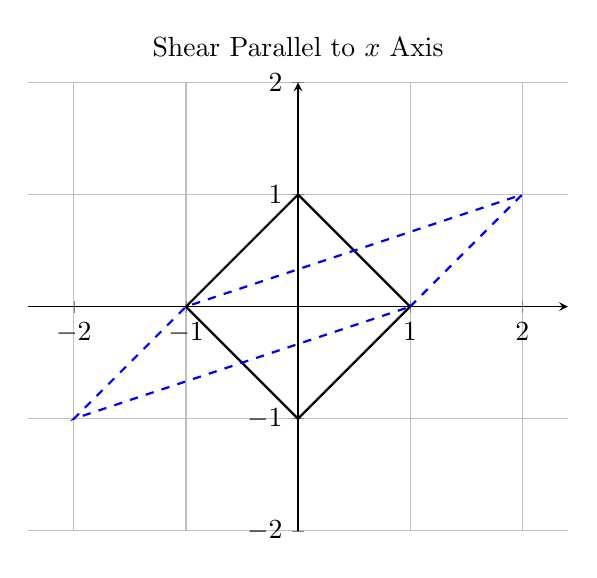
\begin{tikzpicture}
            \begin{axis}[axis equal, axis lines=center, grid, xmin=-2, xmax=2, ymin=-2, ymax=2,
                title={Shear Parallel to $x$ Axis}]
                \draw[thick, black] (axis cs:1,0) -- (axis cs:0,1) -- (axis cs:-1,0) --
                (axis cs:0,-1) -- (axis cs:1,0);
                \draw[thick, dashed, blue] (axis cs:1,0) -- (axis cs:2,1) -- (axis cs:-1,0) --
                (axis cs:-2,-1) -- (axis cs:1,0);
            \end{axis}
        \end{tikzpicture}
        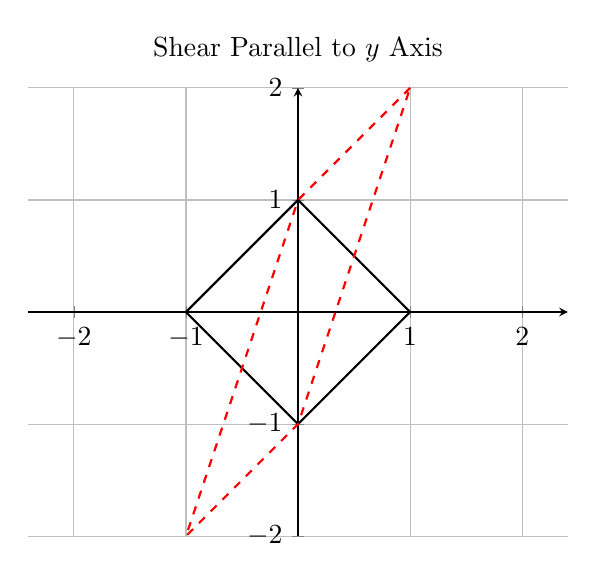
\begin{tikzpicture}
            \begin{axis}[axis equal, axis lines=center, grid, xmin=-2, xmax=2, ymin=-2, ymax=2,
                title={Shear Parallel to $y$ Axis}]
                \draw[thick, black] (axis cs:1,0) -- (axis cs:0,1) -- (axis cs:-1,0) --
                (axis cs:0,-1) -- (axis cs:1,0);
                \draw[thick, dashed, red] (axis cs:1,2) -- (axis cs:0,1) -- (axis cs:-1,-2) --
                (axis cs:0,-1) -- (axis cs:1,2);
            \end{axis}
        \end{tikzpicture}
    \end{center}
    \caption{Examples of shear transformations. The blue transformation on the left is a
    shear parallel to the $x$ axis.  The red transformation on the right is a shear
parallel to the $y$ axis.}
    \label{fig:lt_shear}
\end{figure}

\begin{definition}[Dilation Matrices]
    The 2D linear transformation that geometrically dilates a figures by a factor of $r$ is defined as 
    \[ T(\bx) = \begin{pmatrix} \underline{\hspace{0.25in}} & 0 \\ 0 &
        \underline{\hspace{0.25in}} \end{pmatrix} \bx. \]
    (fill in the blanks)
\end{definition}

\begin{problem}
    In Figure \ref{fig:lt_dilation} we applied two different dilation transformations to the set $S =
    \{(0,0),(1,1),(1,2),(0,1)\}$.  Which dilation transformations were applied?
\end{problem}
\solution{
The left is a dilation by 2 and the right is a dilation by $-0.5$.
}

\begin{figure}[ht!]
    \begin{center}
        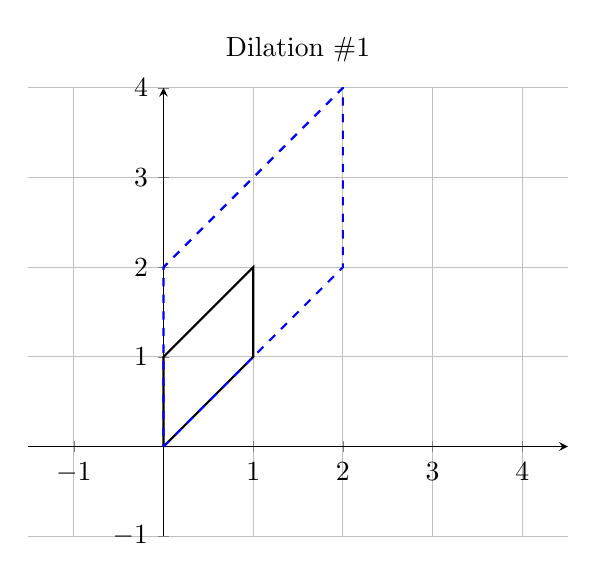
\begin{tikzpicture}
            \begin{axis}[axis equal, axis lines=center, grid, xmin=-1, xmax=4, ymin=-1,
                ymax=4, title={Dilation \#1}]
                \draw[thick, black] (axis cs:0,0) -- (axis cs:1,1) -- (axis cs:1,2) --
                (axis cs:0,1) -- (axis cs:0,0);
                \draw[thick, dashed, blue] (axis cs:0,0) -- (axis cs:2,2) -- (axis cs:2,4) --
                (axis cs:0,2) -- (axis cs:0,0);
            \end{axis}
        \end{tikzpicture}
        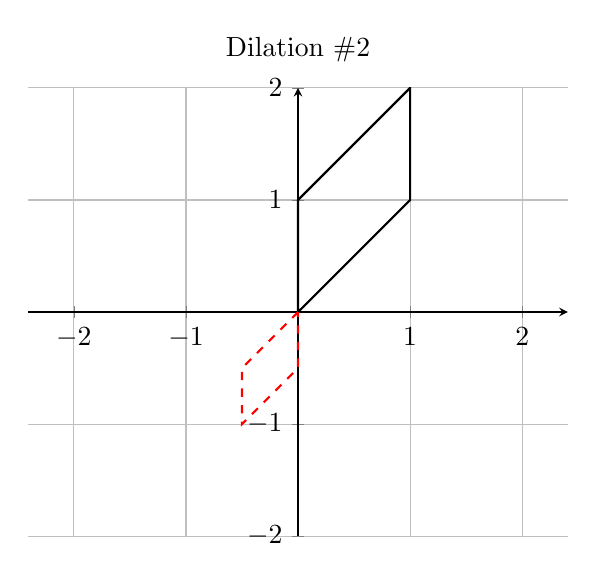
\begin{tikzpicture}
            \begin{axis}[axis equal, axis lines=center, grid, xmin=-2, xmax=2, ymin=-2, ymax=2,
                title={Dilation \#2}]
                \draw[thick, black] (axis cs:0,0) -- (axis cs:1,1) -- (axis cs:1,2) --
                (axis cs:0,1) -- (axis cs:0,0);
                \draw[thick, dashed, red] (axis cs:0,0) -- (axis cs:-0.5,-0.5) -- (axis
                cs:-0.5,-1) -- (axis cs:0,-0.5) -- (axis cs:0,0);
            \end{axis}
        \end{tikzpicture}
    \end{center}
    \caption{Examples of dilation transformations.}
    \label{fig:lt_dilation}
\end{figure}

\begin{definition}[Rotation Matrices]
    The 2D linear transformation that geometrically rotates a figure by an angle $\theta$
    is defined as 
    \[ T(\bx) = \begin{pmatrix} \cos(\theta) & -\sin(\theta) \\ \sin(\theta) &
        \cos(\theta) \end{pmatrix}. \]
\end{definition}

\begin{problem}
    What matrices yield to the following linear transformation?
    \begin{enumerate}
        \item[(a)] A rotation by $90^\circ$ counterclockwise.
        \item[(b)] A rotation by $90^\circ$ clockwise.
        \item[(c)] A rotation by $45^\circ$ counterclockwise.
        \item[(d)] A rotation by $30^\circ$ clockwise.
    \end{enumerate}
\end{problem}


\begin{figure}[ht!]
    \begin{center}
        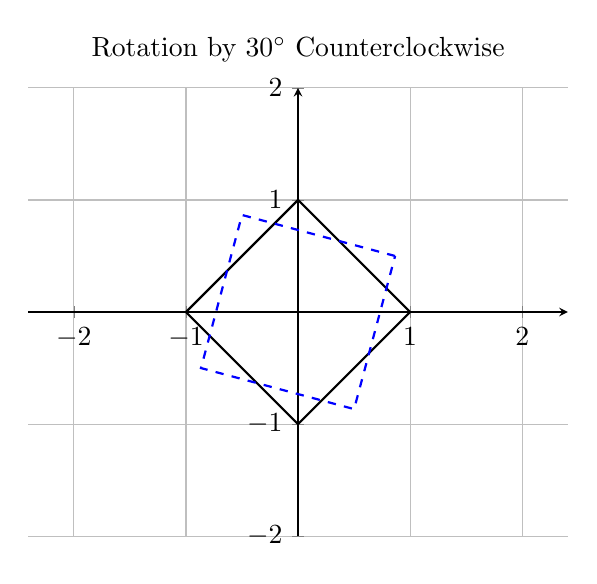
\begin{tikzpicture}
            \begin{axis}[axis equal, axis lines=center, grid, xmin=-2, xmax=2, ymin=-2, ymax=2,
                title={Rotation by $30^\circ$ Counterclockwise}]
                \draw[thick, black] (axis cs:1,0) -- (axis cs:0,1) -- (axis cs:-1,0) --
                (axis cs:0,-1) -- (axis cs:1,0);
                \draw[thick, dashed, blue] (axis cs:0.866,0.5) -- (axis cs:-0.5,0.866) --
                (axis cs:-0.866,-0.5) -- (axis cs:0.5,-0.866) -- (axis cs:0.866,0.5);
            \end{axis}
        \end{tikzpicture}
        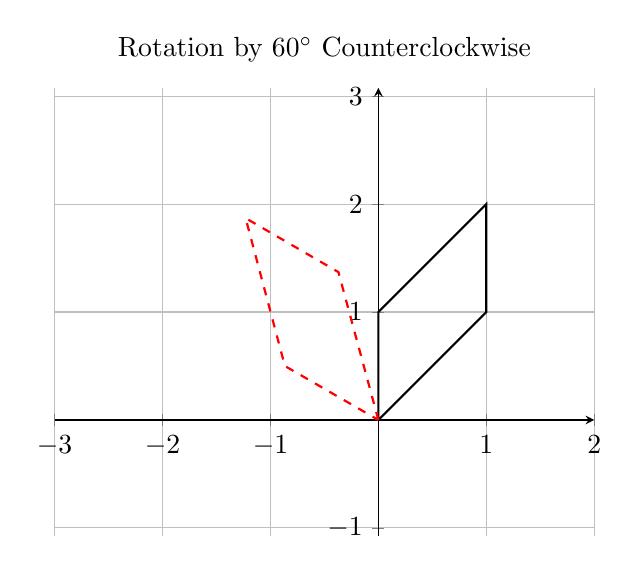
\begin{tikzpicture}
            \begin{axis}[axis equal, axis lines=center, grid, xmin=-3, xmax=2, ymin=-1, ymax=3,
                title={Rotation by $60^\circ$ Counterclockwise}]
                \draw[thick, black] (axis cs:0,0) -- (axis cs:1,1) -- (axis cs:1,2) --
                (axis cs:0,1) -- (axis cs:0,0);
                \draw[thick, dashed, red] (axis cs:0,0) -- (axis cs:-0.37,1.37)
                -- (axis cs:-1.23,1.87) -- (axis cs:-0.866,0.5) -- (axis
                cs:0,0);
            \end{axis}
        \end{tikzpicture}
    \end{center}
    \caption{Examples of rotation transformations. The blue transformation on the left is a
    rotation by $30^\circ$ counterclockwise.  The red transformation on the right is a
rotation by $60^\circ$ counterclockwise.}
    \label{fig:lt_rotation}
\end{figure}

Now that we know the back geometric linear transformations let's see what happens when we
compose several of them.  
\begin{problem}
    Consider the set of points $S = \{(0,0),(1,0),(1,1),(0,1)\}$.  \\(You may want to
    write code to complete this problem)
    \begin{enumerate}
        \item[(a)] Shear the shape generated by $S$ by a factor of 2 parallel to the $x$
            axis and then dilate the resulting shape by a factor of 3.  Draw the resulting
            geometric shape and find the matrix that does these transformations as one
            linear transformation.
        \item[(b)] Dilate the shape generated by $S$ by a factor of 3 and then shear the
            resulting shape by a factor of 2 parallel to the $x$
            axis.  Draw the resulting
            geometric shape and find the matrix that does these transformations as one
            linear transformation.
        \item[(c)] Rotate the shape generated by $S$ by $60^\circ$ counterclockwise, then
            dilate the resulting shape by a factor of $-1.5$, and finally shear the shape
            by a factor of 3 parallel to the $y$ axis.  Draw the resulting
            geometric shape and find the matrix that does these transformations as one
            linear transformation.
    \end{enumerate}
\end{problem}



\subsection{Linear Transformations in Abstract Vector Spaces}
\begin{problem}\label{prob:calc_lt}
    In calculus we know of two very important linear transformations.  Let $\mathcal{V}$
    be the vector space of all real-valued functions $f$ on the interval $[a,b]$ that are
    differentiable and continuous on $[a,b]$.  Let $\mathcal{W}$ be the vector space
    $C[a,b]$ of all continuous functions on $[a,b]$.  
    \begin{itemize}
        \item The transformation $D: \mathcal{V} \to \mathcal{W}$ is defined as $D(f) =
            f'$.  That is, $D$ is the transformation that takes a derivative of a
            function.
        \item The transformation $\mathcal{I}: \mathcal{W} \to \mathcal{V}$ is defined as
            $\mathcal{I}(f) = \int_a^x f(\tau) d\tau$.  That is, $\mathcal{I}$ is the
            transformation that gives the antiderivative of a function.
    \end{itemize}
    Verify that both of these well-known transformations are indeed linear
    transformations.
\end{problem}
\solution{
Pulling scalars and sums around in integrals and derivatives is appropriate.  This is
known from calc 1 but the reason is that these are linear transformations.
}

\begin{definition}[Kernel of a Linear Transformation]
    Let $T$ be a linear transformation from the vector space $\mathcal{V}$ to the vector
    space $\mathcal{W}$.  The {\bf kernel} of T is defined as
    \[ \text{Ker}(T) = \{ \bx \in \mathcal{V} \, : \, T(\bx) = \bo \in \mathcal{W} \}. \]
    Observe that the kernel is another name for the null space.
\end{definition}


\begin{problem}
    Let $D$ be the linear transformation defined as $D(f) = f'$ as in problem
    \ref{prob:calc_lt}.  What is the kernel of $D$?
\end{problem}
\solution{
The set of all constant functions.
}


% \begin{problem}
%     Let $\mathcal{I}$ be the linear transformation defined as $\mathcal{I}(f) = \int_a^x
%     f(\tau) d\tau$ as in problem \ref{prob:calc_lt}.  What is the kernel of $\mathcal{I}$?
% \end{problem}
% \solution{
% We need to get the zero function out so the only thing in the kernel is the zero function.
% }


\begin{problem}
    Define $T(y)$ on $\mathcal{V} = \{y(t) : y'(t) \text{ and } y''(t) \text{ exist } \}$
    and define $T(y) = \frac{d^2y}{dt^2}$.  What is the kernel of $T$?
\end{problem}
\solution{
The set of all linear functions.
}

\begin{problem}
    Define $T: \mathcal{P}_2 \to \mathbb{R}^2$ by 
    \[ T(p) = \begin{pmatrix} p(0) \\ p(1) \end{pmatrix}. \]
    For instance, if $p(t) = 3 + 5t + 7t^2$ then $T(p) = \begin{pmatrix} 3 \\ 15
    \end{pmatrix}$.
    \begin{enumerate}
        \item[(a)] Verify that $T$ is indeed a linear transformation.
        \item[(b)] Find a polynomial $p(x) \in \mathcal{P}_2$ that is in the kernel of $T$.
    \end{enumerate}
\end{problem}
\solution{
    (adapted from 4.2 problem 31 of \cite{Lay}). \\
    \begin{enumerate}
        \item[(a)] $T(c_1 p+c_2 q) = \begin{pmatrix} c_1 p(0) + c_2 q(0) \\ c_1 p(1) + c_2
                q(1) \end{pmatrix} = c_1 \begin{pmatrix} p(0) \\ q(0) \end{pmatrix} + c_2
            \begin{pmatrix} p(1) \\ q(1) \end{pmatrix} = c_1 T(p) + c_2 T(q) $
        \item[(b)] $p(x) = cx-cx^2$ would work just fine.
    \end{enumerate}
}

\begin{problem}
    Let $M_{2\times2}$ be the vector space of all $2 \times 2$ matrices and define $T(A) =
    A + A^T$ for $A \in M_{2 \times 2}$.  Let $B$ be any matrix in $M_{2\times2}$ such
    that $B^T = B$.  Find a matrix $A$ such that $T(A) = B$.  Then describe the kernel of
    $T$.
\end{problem}
\solution{(adapted from 4.2 problem 33 of \cite{Lay}) \\
$A = (1/2) B$\\
The kernel of $T$ consists of matrices of the form $\begin{pmatrix} 0 & a \\ -a & 0
\end{pmatrix}$ where $a \in \mathbb{R}$.
}


\begin{example}
    Determine if the transformation $T: \mathbb{R}^2 \to \mathbb{R}^2$ defined by 
    \[ T\begin{pmatrix} x_1 \\ x_2 \end{pmatrix} = \begin{pmatrix} 4x_1 - 2x_2 \\ 3 |x_2|
    \end{pmatrix} \]
    is or is not a linear transformation.\\
    {\bf Solution:} By the definition of a linear transformation we need to see check that
    $T(\bu + \bv) = T(\bu+\bv)$ and that $T(c\bu) = cT(\bu)$ for arbitrary vectors
    $\bu,\bv\in\mathbb{R}^2$.  

    Let $\bu = \begin{pmatrix} u_1 \\ u_2 \end{pmatrix}$ and $\bv = \begin{pmatrix} v_1 \\
        v_2 \end{pmatrix}$ and observe that 
    \[ T(\bu + \bv) = T\left(\begin{pmatrix} u_1 \\ u_2 \end{pmatrix} + \begin{pmatrix} v_1
        \\ v_2 \end{pmatrix} \right) = T\left( \begin{pmatrix} u_1 + v_1 \\ u_2 + v_2
\end{pmatrix} \right) = \begin{pmatrix} 4(u_1+v_1) - 2(u_2 + v_1) \\ 3 |u_2+v_1|
\end{pmatrix}. \]
    We can clearly separate the first component but due to the absolute value in the
    second component we cannot separate the result of the previous equation to form
    $T(\bu)+T(\bv)$.  Therefore, $T$ is not a linear transformation.
\end{example}

\begin{thm}
    If $T$ is a linear transformation then $T(\bo) = \bo$.
\end{thm}
\begin{proof}
    If $T$ is a linear transformation then $T(c\bu) = cT(\bu)$ for any vector $\bu$ and
    any scalar $c\in\mathbb{R}$.  If we take $c=0$ then $T(0\bu) = cT(\bu)$ which implies
that $T(\bo) = \bo$.
\end{proof}

\begin{example}
   Determine if the transformation $T(x_1,x_2,x_3) = (1,x_2,x_3)$ is a linear
   transformation. \\
   {\bf Solution:} Observe that $T(0,0,0) = (1,0,0)$ so by the previous theorem we see that
   $T$ is not a linear transformation.
\end{example}

\begin{example}
    Determine if the transformation $T(x_1,x_2,x_3) = (x_1,0,x_3)$ is a linear
    transformation. \\
    {\bf Solution:} Since $T(\bo) =\bo$ it is possible that $T$ is a linear transformation
    but we cannot use this to prove that $T$ \underline{is} linear.  We need to check that
    $T(c_1 \bu + c_2 \bv) = c_1 T(\bu) + c_2 T(\bv)$.  Indeed, let $\bu = (u_1,u_2,u_3)$
    and let $\bv = (v_1,v_2,v_3)$ and let $c_1, c_2 \in \mathbb{R}$.  Therefore,
    \[ T(c_1 \bu + c_2 \bv) = T( (c_1 u_1, c_1 u_2, c_1 u_3) + (c_2 v_1, c_2 v_2, c_2
    v_3)) = T( (c_1 u_1 + c_2 v_1, c_1 u_2 + c_2 v_2, c_1 u_3 + c_2 v_3)) \]
    Applying the transformation gives
    \[ T(c_1 \bu + c_2 \bv) = (c_1 u_1 + c_2 v_1, 0, c_1 u_3 + c_2 v_3) =\cdots =  c_1 T(\bu) + c_2
    T(\bv) \]
    which means that $T$ is indeed a linear transformation.
\end{example}

In this class we have studied two particular types of questions: solving first order
non-homogeneous differential equations and solving systems of equations.  Let's consider
the processes for these two problems side by side so that we can truly see them as the
exact same problem in the language of linear transformations.

\begin{minipage}{0.45\columnwidth}
    {\bf Non-homogeneous 1$^{st}$ order ODE}
    \begin{enumerate}
        \item Solve $y' + Py = Q(t)$
        \item Let $T(y) = y'+Py$.  We want to find $y$ so that $T(y) = Q$.
        \item Find $y_h \in \text{Ker}(T)$
        \item Find a particular $y_p$ so that $T(y_p) = Q$.
        \item The solution to $T(y) = Q$ is $y = y_h + y_p$
    \end{enumerate}
\end{minipage}
\begin{minipage}{0.45\columnwidth}
    {\bf Non-homogeneous linear system} 
    \begin{enumerate}
        \item Solve $A \bx = \bb$
        \item Let $T(\bx) = A\bx$.  We want to find $\bx$ so that $T(\bx) = \bb$.
        \item Find $\bx_h \in \text{Null}(A)$
        \item Find a particular $\bx_p$ so that $T(\bx) = \bb$.
        \item The solution to $T(\bx)=\bb$ is $\bx = \bx_h+\bx_p$
    \end{enumerate}
\end{minipage}

\begin{example}
    In this example we will solve two problems related to linear transformations.
    Let $T_1(y) = y'+0.5y$ and $Q(t) = 3$.  Let $T_2(\bx) = \begin{pmatrix} 1 & 3 \\ 2 &
        6 \end{pmatrix} \bx$ and let $\bb = \begin{pmatrix} 5 \\ 10 \end{pmatrix}$.  Solve
            $T_1(y) = Q$ and $T_2(\bx) = \bb$.

\begin{minipage}{0.45\columnwidth}
    {\bf $T_1(y) = Q$}
    \begin{enumerate}
        \item The homogeneous solution is $y_{h} \in \text{span}\{e^{-0.5t}\}$.
        \item The non-homogeneity if a constant function so $y_p \in \text{span}\{1\}$
        \item The solution to $T_1(y) = Q$ is $y = C_0 e^{-0.5t} + C_1$ where $C_0, C_1 \in
            \mathbb{R}$.
    \end{enumerate}
\end{minipage}
\begin{minipage}{0.45\columnwidth}
    {\bf $T_2(\bx) = \bb$}
    \begin{enumerate}
        \item After row reducing the homogeneous solution is $\bx_{h} \in
            \text{span}\left\{ \begin{pmatrix} -3 \\ 1
            \end{pmatrix} \right\}$
        \item After row reducing with $\bb$ on the right we see that the particular
            solution is $\bx_p = \begin{pmatrix} 5 \\ 0 \end{pmatrix}$
            \item The solution to $T_2(\bx)=\bb$ is $\bx = \begin{pmatrix} 5 \\
                    0\end{pmatrix} + \begin{pmatrix} -3 \\ 1 \end{pmatrix} t$ where $t \in
                        \mathbb{R}$.
    \end{enumerate}
\end{minipage}
\end{example}



\begin{example}
    Consider the homogeneous linear differential equation $y' + 0.5 y = 0$.  We can see this as a
    question about the kernel of a linear transformation.  Indeed, if we let $T(y) = y' -
    0.5y$ be a transformation from the space of differentiable functions to the space of
    continuous functions (on appropriate domains) then the differential equation can
    simply be stated as: find $y$ in the kernel of the transformation $T(y) = y' + 0.5y$. 

    The kernel of this linear transformation is spanned by $y(t) = e^{-0.5t}$ since $T(y)
    = 0$.  Therefore the solution to the differential equation is $y(t) = C e^{-0.5t}$.
\end{example}

\begin{problem}
    Consider the homogeneous linear differential equation $y'' + y' - y = 0$.  Rewrite this
    differential equation as a question about the kernel of an appropriate linear
    transformation.
\end{problem}
\solution{
$T(y) = y'' + y' - y$
}

\begin{problem}
    For non-homogeneous linear differential equations we can re-frame them in the language
    of linear transformations in the following way.  
    \begin{itemize}
        \item Find a function in the kernel of the transformation
        \item Find a particular solution that satisfies the non-homogeneous equation
        \item The general solution is a linear combination of the kernel solution and the
            particular solution.
    \end{itemize}
    Use this idea to solve $T(y) = \sin(t)$ where $T(y) = y' + y$
\end{problem}
\solution{
    The kernel of the linear transformation is spanned by $y(t) = e^{-t}$.  Therefore the
    solution is $C_1 e^{-t} + C_1 \sin(t) + C_2 \cos(t)$.
}

\begin{problem}
    Let $T$ be a linear transformation that maps vectors in $\mathbb{R}^2$ to vectors in
    $\mathbb{R}^2$.  Symbolically we write $T: \mathbb{R}^2 \to \mathbb{R}^2$.  Assume
    that 
    \[ T\begin{pmatrix} 1 \\ 0 \end{pmatrix} = \begin{pmatrix} 3 \\ -1 \end{pmatrix} \quad
            \text{and} \quad T\begin{pmatrix} 0 \\ 1 \end{pmatrix} = \begin{pmatrix} -7 \\
                -3 \end{pmatrix}. \]
    Use the following hints to determine the action of $T$ on an arbitrary vector
    $\begin{pmatrix} x_1 \\ x_2 \end{pmatrix} \in \mathbb{R}^2$.
        \begin{itemize}
            \item Expand $\begin{pmatrix}x_1\\x_2\end{pmatrix}$ as a linear combination of
                    the basis vectors $\begin{pmatrix}1\\0\end{pmatrix}$ and
                        $\begin{pmatrix}0\\1\end{pmatrix}$.
            \item Recall that if $T$ is a linear transformation then $T(c \bu) = cT(\bu)$ and
                $T(\bu+\bv) = T(\bu) + T(\bv)$.  Use this fact to write
                $T\begin{pmatrix}x_1\\x_2\end{pmatrix}$
            \item Simplify your answer to give the definition of $T$.
        \end{itemize}
\end{problem}
\solution{
    \begin{flalign*}
        T\begin{pmatrix} x_1 \\ x_2 \end{pmatrix} &= T\left( x_1 \begin{pmatrix}
            1\\0\end{pmatrix} + x_2 \begin{pmatrix} 0 \\ 1 \end{pmatrix} \right) \\
        &= x_1 T\begin{pmatrix} 1\\0\end{pmatrix} + x_2 T\begin{pmatrix}0\\1\end{pmatrix}
            \\
        &= x_1 \begin{pmatrix} 3\\-1\end{pmatrix}  + x_2 \begin{pmatrix} -7 \\
            -3\end{pmatrix} \\
        &= \begin{pmatrix} 3x_1 - 7x_2 \\ -x_1 - 3 x_2 \end{pmatrix}
    \end{flalign*}
}

\begin{thm}\label{thm:transformation_to_basis}
    Let $T: \mathcal{V} \to \mathcal{W}$ be a linear transformation from a vector space
    $\mathcal{V}$ to a vector space $\mathcal{W}$.  The action of $T$ on any vector $\bv
    \in \mathcal{V}$ is completely determined by the actions of $T$ on the basis vectors
    for $\mathcal{V}$.  

    More clearly:\\
    Let $\mathcal{B}=\{\bv_1,\bv_2,\ldots,\bv_k\}$ be a basis for the vector space
    $\mathcal{V}$.  Let $T$ be a linear transformation from $\mathcal{V}$ to vector space
    $\mathcal{W}$ and assume that 
    \[ T(\bv_1) = \bw_1, \quad T(\bv_2) = \bw_2, \quad \ldots \quad T(\bv_k) = \bw_k \]
    where $\bw_1, \bw_2, \ldots, \bw_k \in \mathcal{W}$.  If $\bv$ is written as a linear
    combination of basis vectors from $\mathcal{B}$
    \[ \bv = \sum_{j=1}^k c_j
        \bv_j, \]
    then 
    \[ T(\bv) = \sum_{j=1}^k c_j \bw_j \]
\end{thm}
\begin{proof}
    The proof follows from the definition of a linear transformation.
    \begin{flalign*}
        T(\bv) &= T\left( c_1 \bv_1 + c_2 \bv_2 + \cdots + c_k \bv_k \right) \\
        &= T(c_1 \bv_1) + T(c_2 \bv_2) + \cdots + T(c_k \bv_k) \\
        &= c_1 T(\bv_1) + c_2 T(\bv_2) + \cdots + c_k T(\bv_k) \\
        &= c_1 \bw_1 + c_2 \bw_2 + \cdots + c_k \bw_k
    \end{flalign*}
\end{proof}
The consequence of Theorem \ref{thm:transformation_to_basis} is that all we really need to
know is the action of a linear transformation on the basis vectors and we know the entire
definition of the transformation.\footnote{Note here that we are implicitly assuming that
    the vector spaces $\mathcal{V}$ and $\mathcal{W}$ are finite dimensional.  If they
    were infinite dimensional the theorem will still hold under suitable convergence
conditions.}

\begin{problem}
    Let $T$ be a linear transformation mapping quadratic polynomials to $2\times 2$
    matrices: $T: \mathcal{P}_2 \to M_{2\times2}$.  Recall that the set $\mathcal{B} = \{ 1, x ,x^2\}$
    is a basis for $\mathcal{P}_2$.  If 
    \begin{flalign*}
        T(1) &= \begin{pmatrix} 1 & 0 \\ 0 & 0 \end{pmatrix} \\
        T(x) &= \begin{pmatrix} 0 & 1 \\ 1 & 0 \end{pmatrix} \\
        T(x^2) &= \begin{pmatrix} 0 & 0\\ 0 & 2 \end{pmatrix} 
    \end{flalign*}
    then what is the action of $T$ on the generic quadratic polynomial $T(ax^2 + bx+c)$?
\end{problem}
\solution{
    \begin{flalign*}
        T(ax^2+bx+c)&= aT(x^2) + bT(x) + cT(1) \\
        &= a \begin{pmatrix} 0 & 0 \\ 0 & 2 \end{pmatrix} + b \begin{pmatrix} 0 & 1 \\ 1 &
            0\end{pmatrix} + c \begin{pmatrix} 1 & 0 \\ 0 & 0 \end{pmatrix} \\
        &= \begin{pmatrix} c & b \\ b & 2a \end{pmatrix}
    \end{flalign*}
}


\newpage\section{Isomorphic Vector Spaces}
What we'll explore in this section is
the following bold claim.
\begin{quote}
    Every vector space of dimension $n$ is {\it geometrically the same} as $\mathbb{R}^n$.
\end{quote}
The consequence of this statement is that, in reality, studying any finite dimensional
vector space is the same as studying the Euclidean spaces $\mathbb{R}^n$.

To make this clear let's look at a few examples.  Consider the vector space $\mathcal{V} =
\mathbb{R}^3$ and the vector space $\mathcal{W} = \mathcal{P}_2$ (polynomials of order 2).
We claim that the set of all polynomials of order 2 is really the same vector space as
$\mathbb{R}^3$.

The standard bases for these two vector spaces are
\[ \mathcal{B}_{\mathcal{V}} = \left\{ \begin{pmatrix} 1\\0\\0\end{pmatrix},
    \begin{pmatrix} 0\\1\\0\end{pmatrix}, \begin{pmatrix}0\\0\\1\end{pmatrix} \right\}
    \quad \text{and} \quad \mathcal{B}_{\mathcal{W}} = \left\{ 1,x,x^2 \right\}. \]
Notice that there is a natural mapping between these two bases:
\[ \begin{pmatrix} 1\\0\\0\end{pmatrix} \leftrightarrow 1 \qquad
    \begin{pmatrix}0\\1\\0\end{pmatrix} \leftrightarrow x \qquad
\begin{pmatrix}0\\0\\1\end{pmatrix} \leftrightarrow x^2. \]
Hence if we have any polynomial $p(x) \in \mathcal{P}_2$ we can use this natural mapping
to find the corresponding vector in $\mathbb{R}^3$.  For a specific example, let's take
the polynomial $p(x) = 3x^2 + 5x - 1$.  Explicitly stating $p(x)$ as a linear combination
of basis vectors from the set $\{1,x,x^2\}$ we see that 
\[ p(x) = -1 (1) + 5(x) + 3(x^2), \]
and hence $p(x)$ maps to
\[ p(x) \mapsto -1 \begin{pmatrix}1\\0\\0\end{pmatrix} + 5
\begin{pmatrix}0\\1\\0\end{pmatrix} + 3 \begin{pmatrix}0\\0\\1\end{pmatrix} =
\begin{pmatrix} -1 \\ 5 \\ 3 \end{pmatrix}. \]
That is to say that the polynomial $p(x) = 3x^2 + 5x-1$ in $\mathcal{P}_2$ is the {\it same
vector} as $\begin{pmatrix}-1\\5\\3\end{pmatrix}$ in $\mathbb{R}^3$.

More generally, the polynomial $a_0 + a_1 x + a_2 x^2 \in \mathcal{P}_2$ is the {\it same
vector} as $\begin{pmatrix}a_0\\a_1\\a_2\end{pmatrix} \in \mathbb{R}^3$.  In this way we
can say that any vector in $\mathcal{P}_2$ has a geometric copy in $\mathbb{R}^3$.  

The words {\it geometrically the same} are not very mathematical.  Instead a mathematician
would use the word {\it isomorphic} meaning {\it same form}.  
\begin{definition}[Isomorphism]
    An {\bf isomorphism} is an invertible mapping between two sets. 
\end{definition}

\begin{definition}[Isomorphic Vector Spaces]
    Two vector spaces are said to be {\bf isomorphic} if there is an isomorphic mapping
    between their bases.
\end{definition}
Since the word {\it isomorphic} means {\it same form} we can loosely describe isomorphic
vector spaces as having the same geometric form -- whatever geometry makes sense in one
vector space makes the same sense in the other.

Let's explore another example using our new terminology.  Consider the vector spaces
$\mathbb{R}^4$ and $M_{2 \times 2}$ (the collection of $2 \times 2$ matrices).  The
standard bases for these vector spaces are
\[ \mathcal{B}_{\mathbb{R}^4} = \left\{ \begin{pmatrix}1\\0\\0\\0\end{pmatrix}\,,\,
    \begin{pmatrix}0\\1\\0\\0\end{pmatrix}\,,\,
    \begin{pmatrix}0\\0\\1\\0\end{pmatrix}\,,\,
    \begin{pmatrix}0\\0\\0\\1\end{pmatrix}\right\} \quad \text{and} \quad
    \mathcal{B}_{M_{2 \times 2}} = \left\{ \begin{pmatrix}1&0\\0&0\end{pmatrix}\,,\,
    \begin{pmatrix}0&1\\0&0\end{pmatrix}\,,\,
    \begin{pmatrix}0&0\\1&0\end{pmatrix}\,,\,
    \begin{pmatrix}0&0\\0&1\end{pmatrix}\right\}
\]
and we note that both of these vector spaces are four dimensional.  
There is a clear natural isomorphism between the two basis sets
\[ 
    \begin{pmatrix}1\\0\\0\\0\end{pmatrix} \leftrightarrow
    \begin{pmatrix}1&0\\0&0\end{pmatrix} \quad
    \begin{pmatrix}0\\1\\0\\0\end{pmatrix} \leftrightarrow
    \begin{pmatrix}0&1\\0&0\end{pmatrix} \quad
    \begin{pmatrix}0\\0\\1\\0\end{pmatrix} \leftrightarrow
    \begin{pmatrix}0&0\\1&0\end{pmatrix} \quad
    \begin{pmatrix}0\\0\\0\\1\end{pmatrix} \leftrightarrow
    \begin{pmatrix}0&0\\0&1\end{pmatrix}.
\]
Hence we see that any $2 \times 2$ matrix has an isomorphic copy in $\mathbb{R}^4$ and the
invertible mapping is
\[ \begin{pmatrix} a & b \\ c & d \end{pmatrix} \leftrightarrow \begin{pmatrix}
    a\\b\\c\\d\end{pmatrix}. \]
More specifically, this means that the matrix $\begin{pmatrix} 2&0\\3&-1\end{pmatrix}$ is
geometrically equivalent (isomorphic) to the vector
$\begin{pmatrix}2\\0\\3\\-1\end{pmatrix}$.



\begin{thm}
    Any vector space of dimension $n$ is isomorphic to $\mathbb{R}^n$.
\end{thm}
\begin{proof}
    Let $\mathcal{V}$ be an $n$ dimensional vector space.  From the definition of
    dimension this means that $\mathcal{V}$ has a basis that contains $n$ vectors.  Let
    the basis $\mathcal{B}_{\mathcal{V}}$ be denoted as 
    \[ \mathcal{B}_{\mathcal{V}} = \{ \bv_1, \bv_2, \ldots, \bv_n\}. \]
    The natural isomorphism between the basis for $\mathcal{V}$ and $\mathbb{R}^n$ is
    therefore
    \[ \bv_1 \leftrightarrow \begin{pmatrix}1\\0\\0\\\vdots\\0\end{pmatrix}, \quad \bv_2
    \leftrightarrow \begin{pmatrix}0\\1\\0\\\vdots\\0\end{pmatrix}, \quad \cdots \quad
\bv_n \leftrightarrow \begin{pmatrix} 0\\0\\\vdots\\0\\1\end{pmatrix}. \]
\end{proof}

\begin{problem}
    Show that $\mathcal{P}_3$ (the space of third order polynomials) is isomorphic to
    $M_{2 \times 2}$.
\end{problem}

Now for some fun.
\begin{problem}
    Let $\mathcal{P}_2$ be the vector space of second order polynomials and let $T$ be a linear
    transformation $T:\mathcal{P}_2 \to \mathcal{P}_1$ that maps a quadratic polynomial to its
    derivative (which of course is linear).  For example, $T(3x^2+5x-1) = 6x+5$.
    \begin{enumerate}
        \item[(a)] Using the natural isomorphism between $\mathcal{P}_2$ and
            $\mathbb{R}^3$ map the polynomial $p(x) = 3x^2 + 5x - 1$ to a vector
            $\bu \in \mathbb{R}^3$. 
        \item[(b)] Using the natural isomorphism between $\mathcal{P}_1$ and
            $\mathbb{R}^2$ map the polynomial $q(x) = 6x+5$ to a vector $\bw \in \mathbb{R}^2$.
        \item[(c)] There is a matrix $A$ such that $A \bu = \bw$.  Find it.
        \item[(d)] Use your answer to part (c) to take the derivative of $p(x) = ax^2 + bx
            + c$.  That is: map $p(x)$ to $\mathbb{R}^3$, apply the matrix transformation
            from part (c), then map your answer from $\mathbb{R}^2$ to $\mathcal{P}_1$.
        \item[(e)] The linear transformation $T:\mathcal{P}_{n} \to \mathcal{P}_{n-1}$
            that takes derivatives of $n^{th}$ order polynomials is equivalent to what
            matrix transformation?
        \item[(f)] \ldots stop and think about this for a second \ldots you just showed
            that taking derivatives of a polynomial is really just a matrix operation
            \ldots mind = blown!
    \end{enumerate}
\end{problem}


\begin{problem}
    Come up with a matrix transformation that has the same action as taking an
    antiderivative.
\end{problem}



\begin{problem}
    True or False: The function $h(t) = 4+3t$ is a linear combination of the functions
    $f(t) = (1+t)^2$ and $g(t) = 2 - t - 2t^2$.  Answer this question by using the fact
    that the polynomial spaces are isomorphic to the Euclidean spaces.
\end{problem}
\solution{
True.  $h(t) = 2f(t) + g(t) = 2(1+2t+t^2) + (2-t-2t^2) = 4 + 3t$
}

% \begin{problem}
%     \begin{itemize}
%             \input{ClickerQuestions/LA.00.17.050}
%     \end{itemize}
% \end{problem}

\begin{problem}
    True or False: The function $h(t) = t^2$ is a linear combination of $f(t) = (1-t)^2$
    and $g(t) = (1+t)^2$. Answer this question by using the fact
    that the polynomial spaces are isomorphic to the Euclidean spaces.
\end{problem}
\solution{False}


\begin{problem}
    The dot product in $\mathbb{R}^2$ is easy remember, but now that we know that
    $\mathbb{R}^2$ is isomorphic to the vector space of all linear functions it is natural
    to ask if there is a natural inner product on $\mathcal{P}_1$ that is analogous to the
    dot product.  Let $p(x) = p_0 + p_1x$ and $q(x) = q_0 + q_1 x$.  Map both $p$ and $q$
    to $\mathbb{R}^2$ via the natural isomorphism and take the dot product.  Does the
    resulting formula give a valid inner product on $\mathcal{P}_1$?  You'll need to check
    the following (according to Definition \ref{def:inner_product}).
    \begin{enumerate}
        \item $\left< p,q\right> = \left<q,p\right>$ for $p,q\in\mathcal{P}_1$?
        \item $\left< p,q+r\right> = \left<p,q\right> + \left<p,r\right>$ for
            $p,q,r\in\mathcal{P}_1$?
        \item $\left<cp,q\right> = c\left<p,q\right>$ for $p,q\in\mathcal{P}_1$ and $c \in \mathbb{R}$?
        \item $\left<p,p\right> \ge 0$ and $\left<p,p\right>=0$ iff $p=0$ for $p \in
            \mathcal{P}_1$.
    \end{enumerate}
\end{problem}



\begin{problem}
    Consider the vector space $M_{2\times2}$ of all $2 \times 2$ matrices along with the
    inner product 
    \[ \left<A,B\right> = \text{trace}(AB^T) = \text{trace}\left( 
        \begin{pmatrix} a_{11} & a_{12} \\ 
                        a_{21} & a_{22} \end{pmatrix} 
        \begin{pmatrix} b_{11} & b_{21} \\
        b_{12} & b_{22} \end{pmatrix} \right) = \text{trace}\left( 
        \begin{pmatrix} a_{11} & a_{12} \\ 
                        a_{21} & a_{22} \end{pmatrix} 
        \begin{pmatrix} b_{11} & b_{12} \\
        b_{21} & b_{22} \end{pmatrix}^T \right)\]
    \[ = \text{trace}\left(
                    \begin{pmatrix} a_{11}b_{11} + a_{12} b_{12} & a_{11}b_{21} +
                        a_{12}b_{22} \\ a_{21}b_{11} + a_{22}b_{12} & a_{21} b_{21} +
                    a_{22} b_{22} \end{pmatrix} \right) \]
    \[ = \left( a_{11}b_{11} + a_{12} b_{12} \right) + \left(  a_{21} b_{21} + a_{22}
    b_{22}\right) \]
    \begin{enumerate}
        \item[(a)] Why is this a natural choice for the inner product between $2 \times 2$ matrices?
        \item[(b)] Complete these sentences: 
            \begin{itemize}
                \item Finding the magnitude of $2 \times 2$ matrices with this inner
                    product is geometrically the
                    same as \underline{\hspace{1in}}.
                \item Projecting a $2 \times 2$ matrix onto another $2 \times 2$ matrix is
                    geometrically the same as \underline{\hspace{1in}}.
                \item Finding angles between $2 \times 2$ matrices is geometrically the
                    same as \underline{\hspace{1in}}.
            \end{itemize}
    \end{enumerate}
\end{problem}


\begin{problem}
    An valid inner product on $\mathcal{P}_1[0,1]$ (the set of all linear functions on the
    interval $[0,1]$) is 
    \[ \left<p,q\right> = \int_0^1 p(x) q(x) dx. \]
    Let $p(x) = p_0 + p_1x$ and $q(x) = q_0 + q_1x$ and observe that 
    \begin{flalign*}
        \int_0^1 p(x) q(x) &= \int_0^1 \left( p_0 + p_1 x \right)\left( q_0 + q_1 x
        \right) dx \\
        &= \int_0^1 \left( p_0 q_0 + (p_0 q_1 + p_1 q_0)x + p_1 q_1 x^2 \right) dx \\
        &= \left( p_0 q_0 x + \frac{(p_0 q_1 + p_1 q_0)}{2} x^2 + \frac{p_1 q_1}{3} x^3
        \right)\Big|_0^1 \\
        &= p_0 q_0 + \frac{1}{2}\left( p_0 q_1 + p_1 q_0 \right) + \frac{1}{3} \left( p_1
        q_1
        \right).
    \end{flalign*}
    While this inner product naturally defines a geometry in the space of all linear
    polynomials it doesn't correspond to our usual Euclidean geometry in the isomorphic
    space $\mathbb{R}^2$. That is, if $\bu, \bw \in\mathbb{R}^2$ then we can map both
    vectors to the vector space $\mathcal{P}_1$ via the natural isomorphism and then take
    the inner product via the integral given above.  Since $\mathbb{R}^2$ and
    $\mathcal{P}_1$ are isomorphic they are {\it geometrically equivalent}, but which
    geometry do we get when we use the integral inner product?
    \begin{enumerate}
        \item[(a)] What is the angle between $\begin{pmatrix}1\\0\end{pmatrix}$ and
            $\begin{pmatrix}0\\1\end{pmatrix}$ in this new geometry?  Are these vectors
            still orthogonal?
        \item[(b)] What is the length of the vector $\begin{pmatrix} 1\\1\end{pmatrix}$ in
            this new geometry?
        \item[(c)] If $\bu \perp \bw$ in Euclidean geometry then what do we know about
            them in this new geometry?
        \item[(d)] If $p \perp q$ in $\mathcal{P}_1$ under the integral inner product,
            what does that mean about their images in $\mathbb{R}^2$ under Euclidean
            geometry?
    \end{enumerate}
\end{problem}

The previous two problems should point out an interesting fact about abstract vector spaces: in
many cases the natural geometry from Euclidean space carries over perfectly to the
abstract setting, and sometimes there is more to be gained in the abstract setting an your
Euclidean intuition doesn't hold.  Remember that abstract vector spaces are not
abstractions for the sake of abstractions.  Instead, the content in this chapter was a
revolutionary leap forward in the understanding of mathematics in the 17th century and it
has allowed us to make many modern mathematical discoveries.  It is no exaggeration to say
that 
\begin{quote}
    much of modern mathematics (and hence modern science) is built upon the idea of an
    abstract vector space.
\end{quote}

In this section we have built up the intuition for isomorphic vector spaces by using the
natural standard bases.  We could have also built up these ideas using any other basis and
everything that we've said thus far is true.  The down side to using non-standard bases,
though, is that the notation and subsequent computations becomes more cumbersome.  For a
more in-depth discussion of these ideas see \cite{Lay}.

\newpage\section{Higher Dimensions are Geometrically Weird (Optional)}
At this point you have likely come to the conclusion that linear algebra is beautiful but
possibly very hard to visualize.  This is especially true in more than three dimensions.
In this brief section we'll explore a few strange facts about geometry in higher
dimensions.

\begin{problem}
    Let's first recall some basic geometry but in each of the following problems we'll
    intentionally the language of vector spaces.
    \begin{enumerate}
        \item[(a)] If you are standing at the origin on a 1-dimensional Euclidean vector
            space and you reach out $R$ units in each direction, how much {\it volume} do
            you capture? 
            \solution{You are essentially standing on a number line and you're asked to
                find the amount of the number line from $-R$ to $+R$.  Hence, $V_1 = 2R$
            }
        \item[(b)] If you are standing at the origin of a 2-dimensional Euclidean vector
            space and you reach out $R$ units in every direction, how much {\it volume} do
            you capture?
            \solution{You are now on a plane so the geometric object that you form is a
                circle in the plane.  The {\it volume} of the circle is what we would
                typically call the area: $V_2 = \pi R^2$
            }
        \item[(c)] If you are standing at the origin of a 3-dimensional Euclidean vector
            space and you reach out $R$ units in every direction, how much {\it volume} do
            you capture?
            \solution{You are now in the typical 3 dimensions in which we live so the
                geometric object that you form is a sphere.  The {\it volume} of the
                sphere is: $V_3 =\frac{4}{3} \pi R^3$
            }

    \end{enumerate}
\end{problem}

\begin{problem}
    Now let's make a few conjectures.  Let $V_{n,ball}(R)$ be the volume an
    $n$-dimensional ball of radius $R$ and let $V_{n,cube}(R)$ be the volume of an
    $n$-dimensional cube of side length $2R$.  To make this more concrete, in 2D
    $V_{2,ball}(R)$ is the area of a circle of radius $R$ and $V_{2,cube}(R)$ is the area
    of a square with side length $2R$.  In 3D, $V_{3,ball}(R)$ is the volume of a sphere
    with radius $R$ and $V_{3,cube}(R)$ is the volume of a cube with side length $2R$.
    \begin{enumerate}
        \item[(a)] Without any formal computation, approximately how much area does a
            circle inscribed in a square take up?  In other words, what is $V_{2,ball}(R) /
            V_{2,cube}(R)$?  Verify your conjecture with formal computation.
            \begin{figure}[ht!]
                \begin{center}
                    
\begin{tikzpicture}
                        \draw[thick, black] (-1,-1) -- (1,-1) -- (1,1) -- (-1,1) -- cycle;
                        \draw[thick, fill = red, color=red] (0,0) circle(1cm);
                    \end{tikzpicture}
                \end{center}
                \caption{A circle inscribed in a square.  The ratio of the area of the
                    square to the area of the circle is $V_{2,ball}/V_{2,cube}$.}
                \label{fig:circle_square}
            \end{figure}
        \item[(b)] Without any formal computation, approximately how much area does a
            sphere inscribed in a cube take up?  In other words, what is $V_{3,ball}(R) /
            V_{3,cube}(R)$?  Verify your conjecture with formal computation.
        \item[(c)] Make a conjecture for the value of the limit:
            \[ \lim_{n\to\infty} \frac{V_{n,ball}(R)}{V_{n,cube}(R)}. \]
    \end{enumerate}
\end{problem}


In higher dimensions (4D and up) we have a hard time visualizing anything without using
tricks such as color or time-like variables.  
\begin{definition}[Volume of an $n$-Dimensional Ball]
    For the volume of an $n$-dimensional ball we
    have the recursive formula 
    \begin{flalign}
        V_n(R) = \frac{2\pi R^2}{n} V_{n-2}(R)
        \label{eqn:n_ball_volume}
    \end{flalign}
    where $n$ is the dimension and $R$ is the radius.  
\end{definition}

\begin{problem}
    Given that $V_1 = 2R$ and $V_2 = \pi R^2$, use the recursive formula
    \eqref{eqn:n_ball_volume} to verify the formula for the volume of a
    sphere of radius $R$.
    \[ V_3(R) = \underline{\hspace{1in}} \]
\end{problem}
\solution{
    \[ V_3(R) = \frac{2 \pi R^2}{3} \cdot V_1(R) = \frac{2\pi R^2}{3} \cdot \left( 2R
        \right) = \frac{4}{3} \pi R^3 \]
}

\begin{definition}[Volume of an $n$-Dimensional Cube]
    For a cube of $n$ dimensions with side length $2R$ we always have the simple formula
    \begin{flalign}
        V_n(R) = (2R)^n = 2^n R^n.
        \label{eqn:n_cube_volume}
    \end{flalign}
\end{definition}
A moment's reflection reveals that in a one dimension Euclidean vector space the volume of a
cube and the volume of the sphere are the same: $V_{1,ball} = V_{1,cube} = 2R$.  In two dimensions we have 
\begin{flalign*}
    V_{2,square} &= (2R)^2 = 4R^2 \quad \text{and} \\
    V_{2,circle} &= \pi R^2,
\end{flalign*}
which implies that the fraction of the volume of the square filled by the inscribed circle
is
\[ \frac{V_{2,circle}}{V_{2,square}} = \frac{\pi R^2}{4 R^2} =\frac{\pi}{4} \approx 0.785 \]
so the circle fills approximately 78.5\% of the square. Examining Figure
\ref{fig:circle_square} visually should verify that this {\it appears to be} correct.

In three spatial dimension we have
\begin{flalign*}
    V_{3,cube} &= (2R)^3 = 8R^3 \quad \text{and} \\
    V_{3,sphere} &= \frac{4}{3} \pi R^3,
\end{flalign*}
which implies that 
\[ \frac{V_{3,sphere}}{V_{3,cube}} = \frac{\frac{4}{3} \pi R^3}{8 R^3} =
    \frac{\frac{4}{3} \pi}{8} = \frac{\pi}{6} \approx 0.524 \]
so we see that a sphere inscribed in a cube fills up about 52.4\% of the available volume.
These results are summarized in the table below.

\begin{center}
    \begin{tabular}{|c|c|c|c|}
        \hline
        Dimension ($n$) & Volume of a Ball & Volume of a Cube & Ratio: ($V_{n,ball} /
        V_{n,cube}$) \\ \hline \hline
        1 & $2R$ & $2R$ & $1$ \\ \hline
        2 & $\pi R^2$ & $4R^2$ & $\frac{\pi}{4} \approx 0.785$ \\ \hline
        3 & $\frac{4}{3} \pi R^3$ & $8R^3$ & $\frac{\pi}{6} \approx 0.524$ \\ \hline
        4 & $\frac{2\pi R^2}{4} \cdot \left( \pi R^2 \right) = \frac{\pi^2 R^4}{2} $ &
        $16R^4$ & $\frac{\pi^2}{32} \approx 0.308$ \\ \hline
        5 & $\frac{2\pi R^2}{5} \cdot \frac{4}{3} \pi R^3 = \frac{8 \pi^2 R^5}{15}$ &
        $32R^5$ & $\frac{\pi^2}{60} \approx 0.164$ \\ \hline
        6 &  &  &  \\ \hline
        7 &  &  &  \\ \hline
        8 &  &  &  \\ \hline
        $\vdots$ &  &  &  \\ \hline
    \end{tabular}
\end{center}

\begin{problem}
    The previous table shows the ratio $V_{n,ball} / V_{n,cube}$ for dimensions $1$
    through $5$.  Use equations \eqref{eqn:n_ball_volume} and \eqref{eqn:n_cube_volume} to
    complete the computation for dimensions $6$ - $8$ and conjecture the
    value of 
    \[ \lim_{n \to \infty} \frac{V_{n,ball}(R)}{V_{n,cube}(R)}. \]
    Explain the meaning of the limit geometrically (however counterintuitive it is).
\end{problem}
\solution{
    In the limit, the ratio $V_{n,ball}/V_{n,cube}$ goes to zero.  Geometrically this
    means that a ball of radius $R$ takes up less and less space in a cube of side length
    $2R$ as the dimension increases.  In an infinite dimensional space, a ball of radius
    $R$ takes up zero volume.
\begin{center}
    \begin{tabular}{|c|c|c|c|}
        \hline
        Dimension ($n$) & Volume of a Ball & Volume of a Cube & Ratio: ($V_{n,ball} /
        V_{n,cube}$) \\ \hline \hline
        1 & $2R$ & $2R$ & $1$ \\ \hline
        2 & $\pi R^2$ & $4R^2$ & $\frac{\pi}{4} \approx 0.785$ \\ \hline
        3 & $\frac{4}{3} \pi R^3$ & $8R^3$ & $\frac{\pi}{6} \approx 0.524$ \\ \hline
        4 & $\frac{2\pi R^2}{4} \cdot \left( \pi R^2 \right) = \frac{\pi^2 R^4}{2} $ &
        $16R^4$ & $\frac{\pi^2}{32} \approx 0.308$ \\ \hline
        5 & $\frac{2\pi R^2}{5} \cdot \frac{4}{3} \pi R^3 = \frac{8 \pi^2 R^5}{15}$ &
        $32R^5$ & $\frac{\pi^2}{60} \approx 0.164$ \\ \hline
        6 & $\frac{\pi^3}{6} R^6$ & $64R^6$ & $\frac{pi^3}{384} \approx 0.0807$  \\ \hline
        7 & $\frac{16 \pi^3}{105} R^7$ & $128 R^7$  & $\frac{16 \pi^3}{13440} \approx
        0.0369$  \\ \hline
        8 & $\frac{\pi^4}{24} R^8$ & $256 R^8$  & $\frac{\pi^4}{6144} \approx 0.0159$ \\ \hline
        $\vdots$ &  &  &  \\ \hline
    \end{tabular}
\end{center}
}   


\begin{problem}
    If you want to see a cool video about higher dimensional visualization, check out this
    one by {\it 3 Blue 1 Brown:}
    \href{https://youtu.be/zwAD6dRSVyI}{https://youtu.be/zwAD6dRSVyI}.
\end{problem}

\newpage\section{Additional Exercises}


\begin{problem}[Legendre Polynomials]
   Consider the vector space  
   \[ \mathcal{V} = \{a_0 + a_1 x + a_2 x^2 \, : \, a_0, a_1, a_2 \in
       \mathbb{R} \text{ and } x \in [-1,1] \} \]
    along with the inner product 
    \[ \left< f,g\right> = \int_{-1}^1 f(x) g(x) dx \]
    Consider the basis $\mathcal{B} = \{1,x,\frac{1}{2}(3x^2-1)\}$.  
    \begin{enumerate}
        \item[(a)] Is this basis an orthogonal basis?
        \item[(b)] Set up the necessary calculus to write $h(x) = 3x^2+2$ as a linear
            combination of vectors in $\mathcal{B}$.
    \end{enumerate}
\end{problem}
\solution{This is an orthogonal basis.  We need to consider that
    \[ c_1 (1) + c_2 ( x) + c_3 ( \frac{1}{2} (3x^2-1) ) = h(x) \]
    Since this is an orthogonal basis we can get each $c_j$ by doing
    inner products:
    \begin{flalign*}
        c_1 &= \frac{\left<h(x),1\right>}{\left<1,1\right>}=3 \\
        c_2 &= \frac{\left<h(x),x\right>}{\left<x,x\right>}=0 \\
        c_3 &=
        \frac{\left<h(x),\frac{1}{2}(3x^2-1)\right>}{\left<\frac{1}{2}(3x^2-1),\frac{1}{2}(3x^2-1)\right>}=2 \\
    \end{flalign*}
}                    


\begin{problem}
        The set $S$ below contains three linearly independent mutually orthogonal vectors
        and as such we know that $\text{span}(S) = \mathbb{R}^3$
        \[ S = \left\{ \begin{pmatrix} 3 \\ 1 \\ 1 \end{pmatrix} \, , \, \begin{pmatrix}
                -1 \\ 2 \\ 1 \end{pmatrix} \, , \, \begin{pmatrix} -1 \\ -4 \\ 7
        \end{pmatrix} \right\} \]
        Write the vector $\bu = \begin{pmatrix} 3 \\ 0 \\ 5 \end{pmatrix}$ as a linear
        combination of the vectors in $S$.
\end{problem}
\solution{
    \[ \bu = c_1 \bv_1 + c_2 \bv_2 + c_3 \bv_3 \]
    where $\bv_1, \bv_2, \bv_3 \in S$.  Since the vectors in $S$ are mutually
    orthogonal we have
    \begin{flalign*}
        c_1 &= \frac{\bu \cdot \bv_1 }{\bv_1 \cdot \bv_1} = \frac{14}{11} \\
        c_2 &= \frac{\bu\cdot \bv_2}{\bv_2 \cdot \bv_2} = \frac{2}{6} =
        \frac{1}{3} \\
        c_3 &= \frac{\bu\cdot \bv_3}{\bv_3 \cdot \bv_3} = \frac{32}{66}
        =\frac{16}{33}
    \end{flalign*}
    Therefore
    \[ \bu = \frac{14}{11} \begin{pmatrix} 3 \\ 1 \\ 1 \end{pmatrix} +
            \frac{1}{3} \begin{pmatrix} -1 \\ 2 \\ 1 \end{pmatrix} +
                \frac{16}{33} \begin{pmatrix} -1 \\ -4 \\ 7 \end{pmatrix} \]
                }

\begin{problem}
Let $\mathcal{V} = C[-1,1]$ be the vector space of continuous functions on the closed
interval $[-1,1]$.  An inner product on this vector space is $\left< f,g\right> =
\int_{-1}^1 f(x) g(x) dx$.  

        Let $f(x) = x^2 + 1$ and $g(x) = x$.  Set up (\underline{but do not evaluate}) the
        integrals to find the angle between these two functions in $C[-1,1]$.  
\end{problem}
\solution{
    \begin{flalign*}
        \| f \| &= \sqrt{ \int_{-1}^1 (x^2+1)^2 dx} \\
        \| g \| &= \sqrt{ \int_{-1}^1 x^2 dx } \\
        \left< f , g\right> &= \int_{-1}^1 (x^2+1)(x) dx \\
        \cos(\theta) &= \frac{\left< f , g \right> }{\|x^2+1\| \|x\|}
    \end{flalign*}
}

\begin{problem}
    If $A$ and $B$ are arbitrary $m \times n$ matrices, then the mapping $\left<
    A,B\right> = \text{trace}(A^TB)$ defines an inner product in $\mathbb{R}^{m\times n}$.
    Use this inner product to find $\left<A,B\right>$, the norms, $\|A\|$ and $\|B\|$, and
    the angle between $A$ and $B$ for
    \[ A = \begin{pmatrix} -2 & 3 \\ -1 & 3 \\ 1 & -2 \end{pmatrix} \quad \text{and} \quad
            B = \begin{pmatrix} -2 & 1 \\ 1 & 2 \\ 1 & 1 \end{pmatrix}. \]
\end{problem}
\solution{
    Hint: Recall that for $\bv \in \mathcal{V}$ we have $\|\bv\| = \left< \bv,\bv\right>$
    and if $\bw \in \mathcal{V}$ then the angle between $\bv$ and $\bw$ is defined as
$\left< \bv,\bw\right> = \|\bv\| \|\bw\| \cos\theta$.
}

\begin{problem}
    Find a non-trivial vector that is perpendicular to both $\bv$ and $\bu$ where
    \[ \bv = \begin{pmatrix} 2 \\ 5 \\ 3 \end{pmatrix} \quad \text{ and } \quad \bu =
            \begin{pmatrix} -1 \\ -2 \\ -2 \end{pmatrix} \]
\end{problem}
\solution{
    Hint: Use the Gram-Schmidt process.
}

\begin{problem}
    Determine which of the following transformations are linear transformations.
    \begin{flalign*}
        T_1(x,y,z) &= (x,y,-z) \\
        T_2(x,y) &= (2x-3y,x+4,5y) \\
        T_3(x,y,z) &= (1,y,-z) \\
        T_4(x,y) &= (4x-2y,3|y|) \\
        T_5(x,y,z) &= (x,0,z) 
    \end{flalign*}
\end{problem}
\solution{
    Hint: check out the exact definition of a linear transformation.
}

\begin{problem}
    Let $T: \mathbb{R}^2 \to \mathbb{R}^2$ be a linear transformation that sends the
    vector $\bu = \begin{pmatrix} 5\\2\end{pmatrix}$ to $\begin{pmatrix}
        2\\1\end{pmatrix}$ and maps $\bv = \begin{pmatrix}1\\3\end{pmatrix}$ to
            $\begin{pmatrix} -1\\3\end{pmatrix}$.  Use properties of linear
                transformations to calculate the following.
    \begin{enumerate}
        \item[(a)] $T(-3\bu)$
        \item[(b)] $T(8\bv)$
        \item[(c)] $T(-3\bu + 8\bv)$
    \end{enumerate}
\end{problem}
\solution{
    Hint: recall that in a linear transformation, $T(a\bv) = aT(\bv)$ and $T(\bv+\bu) =
    T(\bv) + T(\bu)$.
}


\begin{problem}
    Let $e_1 = \begin{pmatrix}1\\0\end{pmatrix}$ and $e_2 =
        \begin{pmatrix}0\\1\end{pmatrix}$.  Let $\bv = \begin{pmatrix}-3\\9\end{pmatrix}$ and let $\bu =
            \begin{pmatrix}-5\\-8\end{pmatrix}$.
    If $T:\mathbb{R}^2 \to \mathbb{R}^2$ is a linear transformation that sends $e_1$ to
    $\bv$ and $e_2$ to $\bu$.  Where does $T$ send $\begin{pmatrix}-4\\6\end{pmatrix}$?
\end{problem}
\solution{
    Hint: Start by writing $(-4,6)$ as a linear combination of $e_1$ and $e_2$.
}


\begin{problem}
    Let $T:\mathcal{P}_2 \to \mathcal{P}_2$ be a linear transformation mapping quadratic
    functions to quadratic functions.  Assume that 
    \[ T(1) = 4x^2 + 4, \quad T(x) = 4x+3, \quad \text{and} \quad T(x^2) = 4x^2 + x + 3.
        \]
    Find the image of an arbitrary quadratic polynomial $ax^2 + bx + c$ under $T$.  That
    is, find $T(ax^2 + bx + c)$.
\end{problem}
\solution{
    Hint: Apply the fact that $T$ is a linear transformation to $T(ax^2 + bx + c)$ to
    first get 
    \[ T(ax^2 + bx + c) = aT(x^) + bT(x) + cT(1). \]
    Then apply the transformation given above and simplify.
}




\begin{problem}
    Assume that $T: \mathbb{R}^2 \to \mathbb{R}^2$ is a linear transformation and $T(\bv)
    = \begin{pmatrix} 2&0\\0&1\end{pmatrix}\begin{pmatrix}0&1\\-1&0\end{pmatrix} \bv$.
    \begin{enumerate}
        \item[(a)] Which of the following best describes what $T$ does to the plane?
            \begin{itemize}
                \item $T$ stretches vectors vertically by a factor of 2, then rotates them
                    $90^\circ$ clockwise.
                \item $T$ rotates vectors $90^\circ$ clockwise, then stretches them
                    vertically by a factor of 2.
                \item $T$ stretches vectors horizontally by a factor of 2, then rotates them
                    $90^\circ$ clockwise.
                \item $T$ rotates vectors $90^\circ$ clockwise, then stretches them
                    horizontally by a factor of 2.
            \end{itemize}
        \item[(b)] Explain your choices from part (a)
    \end{enumerate}
\end{problem}

